%% FL-Iroh -- Elsevier CAS (cas-dc) double-column manuscript (ANONYMOUS FOR BLIND REVIEW)
%% Ported from paper.tex (IEEEtran). English only.
%% Compile from this directory so the cas-dc.cls / cas-common.sty are found.

\documentclass[a4paper,fleqn]{cas-dc}

% cas-dc already loads: graphicx, amsmath/amsfonts/amssymb, booktabs,
% makecell, multirow, array, colortbl, dcolumn, xcolor(svgnames,dvipsnames),
% hyperref(colorlinks), fontenc(T1). Do NOT reload those.

\usepackage[utf8]{inputenc}
\usepackage[numbers]{natbib}   % numeric [n] citations, matches thebibliography
\usepackage{tikz}
\usetikzlibrary{arrows.meta, positioning, shapes.geometric, calc}
\usepackage{pgfplots}
\pgfplotsset{compat=1.18}
\graphicspath{{../../../img/}}

% Absorb minor overfull \hbox boxes in the narrow two-column measure
\emergencystretch=3em
\tolerance=800

\begin{document}
\let\WriteBookmarks\relax
\def\floatpagepagefraction{1}
\def\textpagefraction{.001}

\shorttitle{FL-Iroh: NAT-Transparent Federated Learning for Agricultural and Environmental IoT}
\shortauthors{Anonymous}

\title[mode = title]{FL-Iroh: NAT-Transparent Federated Learning for Agricultural and Environmental IoT via QUIC P2P Transport and CoAP Service Discovery}

% ---- Authors (Anonymous for blind review) --------------------------------
\author{Anonymous Submission}

% ---- Abstract -------------------------------------------------------------
\begin{abstract}
Federated Learning (FL) for agricultural and environmental IoT faces a connectivity barrier: edge devices behind Network Address Translators (NAT) and Carrier-Grade NAT (CGNAT) cannot host or reliably reach an aggregator without static IPs, VPN overlays, or cloud relays. We present FL-Iroh, an open-source FL system that embeds NAT traversal in the application transport: the Iroh QUIC peer-to-peer transport addresses and authenticates peers by Ed25519 public key, a public-key allow-list enforces federation membership, an end-to-end-encrypted relay carries traffic whenever no direct path is validated, and a CoAP/CoRE control plane with a resource directory provides capability-based discovery. We evaluate it on real hardware across three networks (four NAT vantage points) with RFC~4787-classified NAT behavior, including a mobile-carrier CGNAT, with a Raspberry Pi~3B client. All 30 cold starts on a new office--home path and 95.8\% of 120 earlier WAN attempts connected; long-lived sessions used validated direct paths (60/60 transfers), and with all UDP blocked the relay delivered 190/190 transfers, returning to direct within 4~s of unblocking. A federation over the WAN completed 29 of 30 rounds with the Raspberry Pi training in every round it joined (1.0~s and 419~MB peak memory per round); unauthorized peers were rejected in 0.3~s; all 320 rounds of a loss/latency/bandwidth sweep completed; and resource-directory discovery answered multi-tag queries over 5{,}000 endpoints in 19~ms. The transport is aggregation-agnostic, carrying neural networks and a federated Prophet model evaluated with imbalance-aware metrics on air-quality forecasting.
\end{abstract}

\begin{highlights}
\item FL transport with built-in NAT traversal, public-key addressing and admission control
\item RFC~4787-classified networks incl.\ mobile CGNAT; relay delivers 100\% without UDP
\item Real WAN federation with a Raspberry Pi~3B client; CPU, memory and energy per round
\item CoAP resource directory: multi-tag discovery over 5{,}000 endpoints in tens of ms
\item All rounds complete under loss, latency and bandwidth limits typical of rural links
\end{highlights}

\begin{keywords}
Federated Learning \sep NAT Traversal \sep QUIC \sep CoAP \sep Edge Computing \sep Smart Agriculture
\end{keywords}

\maketitle

% ---- Abbreviations (R2.3) -------------------------------------------------
\begin{table}[!t]
\caption{Abbreviations used in this paper}
\label{tab:abbrev}
\scriptsize
\setlength{\tabcolsep}{3pt}
\begin{tabular}{@{}l p{2.9cm} l p{2.9cm}@{}}
\toprule
ALPN & Application-Layer Protocol Negotiation & ICA & \'Indice de Calidad del Aire (Spanish air-quality index) \\
CBOR & Concise Binary Object Representation & IID & Independent and identically distributed \\
CGNAT & Carrier-Grade NAT & IoT & Internet of Things \\
CoAP & Constrained Application Protocol & MLP & Multilayer perceptron \\
CoRE & Constrained RESTful Environments & NAT & Network Address Translation \\
DERP & Designated Encrypted Relay for Packets & QUIC & QUIC transport protocol (RFC~9000) \\
DP & Differential privacy & RD & Resource Directory (RFC~9176) \\
EIM & Endpoint-independent mapping & RSS & Resident set size (memory) \\
FedAvg & Federated Averaging & RTT & Round-trip time \\
FedGAM & Partial aggregation for GAMs & STUN & Session Traversal Utilities for NAT \\
FL & Federated Learning & TLS & Transport Layer Security \\
GAM & Generalized Additive Model & UDP & User Datagram Protocol \\
\bottomrule
\end{tabular}
\end{table}

% =========================================================================
\section{Introduction}
\label{sec:introduction}

Precision agriculture increasingly relies on distributed IoT sensor networks to collect soil chemistry, microclimate, and crop health data. Federated Learning (FL)~\cite{mcmahan2017} offers an appealing paradigm for this domain: individual farms can collaboratively train shared crop recommendation or disease detection models without transmitting raw agronomic data off-site, which keeps raw data local and saves bandwidth on typically constrained rural links.

However, a practical infrastructure barrier stands in the way: the vast majority of agricultural IoT deployments operate behind NAT or CGNAT, with no publicly reachable IP address. Mainstream FL frameworks such as Flower~\cite{flower2022}, TensorFlow Federated~\cite{tff2019}, and FedML~\cite{fedml2020} follow a client-initiated star topology, so NAT-constrained \emph{clients} can participate---but the aggregation \emph{server} must remain publicly reachable. A rented cloud VPS can provide such an endpoint; what it cannot provide is (i)~an aggregator hosted on-premises (e.g., at a farm or cooperative) behind CGNAT, as data-sovereignty and cost considerations often demand; (ii)~a stable server identity that survives IP churn on rural fixed and cellular links; or (iii)~operation without a third-party host that must be provisioned, paid for, secured, and kept alive. For unattended, solar-powered deployments with no administrator on site, these operational requirements---rather than the monthly price of a VPS---are the obstacle.

The \emph{hole-punching} technique~\cite{ford2005}, used by consumer P2P applications, can establish direct UDP connections between NATted peers without dedicated infrastructure. With QUIC~\cite{rfc9000} as the transport, a hole-punched path also carries encrypted, multiplexed streams. Its success depends on how each NAT maps and filters traffic (RFC~4787~\cite{rfc4787}): endpoint-independent mappings are readily traversed, while address- and port-dependent mappings---common in mobile and shared rural broadband---may defeat it. A \emph{relay} with a public IP is therefore needed as a fallback. Unlike a conventional proxy, the DERP (Designated Encrypted Relay for Packets) relay used by Iroh forwards only end-to-end-encrypted traffic, so it never sees model parameters in plaintext. Fig.~\ref{fig:holepunch} illustrates both paths. Existing FL systems provide no integrated mechanism for this fallback.

\begin{figure}[t]
\centering
\includegraphics[width=\columnwidth]{NAT-hole-punching.png}
\caption{NAT hole-punching between two peers on private addresses. \textcircled{\scriptsize 1}~Both peers register with a public signaling/rendezvous server through their NATs; \textcircled{\scriptsize 2}~the server relays to each peer the other's public NAT mapping (address:port); \textcircled{\scriptsize 3}~simultaneous outbound packets open pinholes in both NATs and traffic then flows directly between the peers' public endpoints. In FL-Iroh the rendezvous role is played by the DERP relay, which additionally carries the end-to-end-encrypted traffic whenever a direct path cannot be validated; the application is unaware of which path is active (\S\ref{sec:e3}, \S\ref{sec:e8}).}
\label{fig:holepunch}
\end{figure}

We address this gap with \textbf{FL-Iroh}, a system that integrates:

\begin{enumerate}
    \item \textbf{Iroh}~\cite{iroh2024}, a QUIC-based P2P transport library that implements the DERP relay protocol~\cite{tailscale2023}: hole-punching is attempted first; while no direct path is validated, traffic is relayed through a DERP server with end-to-end encryption, and the session migrates to the direct path once it is validated.
    \item \textbf{CoAP/CoRE}~\cite{rfc7252} as a lightweight control plane with an RFC~9176-style resource directory~\cite{rfc9176} for capability-based client discovery and round coordination, using CBOR serialization on constrained links; for peers that are not mutually reachable at the IP level, registration is carried over an authenticated Iroh control stream instead.
    \item \textbf{Public-key federation membership}: every node is identified by a persistent Ed25519 key, and the aggregator admits only allow-listed keys at the transport level, before any model exchange.
\end{enumerate}

The data plane is independent of IP addressing and of the aggregation rule: it carries the serialized parameters of any model without interpreting them, so changing the aggregation (FedAvg, partial aggregation for GAMs, or others) requires no transport change. It is not, however, independent of the client runtime: the current client requires a Python/PyTorch environment on Cortex-A class devices (\S\ref{sec:agnostic}).

Our primary application domain is agricultural and environmental IoT: soil-based crop recommendation and seven-day-ahead outdoor air-quality forecasting with lightweight models suited to single-board edge computers such as the Raspberry Pi~3B used in our hardware experiments.

\noindent\textbf{Contributions:}
\begin{enumerate}
    \item We design and implement FL-Iroh, an open-source FL architecture that embeds NAT traversal in the application-level transport---an Iroh\slash QUIC data plane with public-key addressing, transport-level admission control, transfer retry and endpoint recovery---coordinated by a CoAP\slash CBOR control plane with a resource directory (\S\ref{sec:system}). The NAT-traversal machinery is provided by the Iroh library~\cite{iroh2024}; our contribution is its integration into, hardening for, and evaluation as an FL substrate.
    \item We provide an empirical connectivity characterization on real hardware across three networks (four NAT vantage points) with RFC~4787-classified NAT behavior---including a mobile-carrier CGNAT---covering cold-start establishment, path validation in long-lived sessions, forced relay operation, link outages and network switches (\S\ref{sec:e3}, \S\ref{sec:e8}). We distinguish validated direct paths from relay-carried ones, a distinction that our earlier analysis had conflated.
    \item We evaluate FL-Iroh end to end: convergence and churn (E2, E4), CoAP discovery scaling to 5{,}000 endpoints (E5), a two-domain application study with imbalance-aware metrics (E6), a packet-loss/latency/bandwidth sweep (E9), admission control (E10), and a complete federation over the WAN with a Raspberry Pi~3B client, including per-round CPU, memory and energy (E11).
\end{enumerate}

We also include a case study of a partial-aggregation rule for Prophet GAMs (FedGAM). A same-model ablation shows that it is statistically indistinguishable from FedAvg on our data, so we present it as an illustration of aggregation-agnostic transport rather than as a contribution in its own right (\S\ref{sec:e6}).

The remainder of this paper is organized as follows. Section~\ref{sec:related} reviews related work. Section~\ref{sec:system} presents the FL-Iroh architecture and protocols. Section~\ref{sec:evaluation} reports the experimental evaluation. Section~\ref{sec:discussion} discusses implications, the security model, and limitations. Section~\ref{sec:conclusion} concludes and outlines a research roadmap.

% =========================================================================
\section{Related Work}
\label{sec:related}

We organize prior work along six axes---FL in agriculture and environmental monitoring, communication-efficient and resource-aware FL, NAT traversal, lightweight IoT protocols for FL, FL over overlays, and decentralized FL---and close with a structured comparison (Table~\ref{tab:related}).

\subsection{Federated Learning for Agricultural and Environmental IoT}

FL has been applied across the agri-food sector, from cross-silo data sharing among stakeholders~\cite{durrant2022} and federated intrusion detection for agricultural IoT~\cite{friha2022} to crop-yield prediction with encrypted gradients in an edge--cloud hierarchy~\cite{dey2025}, nitrous-oxide emission prediction on a farm-deployed IoT/fog architecture~\cite{killeen2025}, and leaf-disease detection with pruned attention networks~\cite{piccialli2025}. In environmental monitoring, federated models forecast PM2.5 across city-level edge servers~\cite{hu2024} and air-quality indices with energy-aware training~\cite{dey2026}, and detect anomalies in environmental sensor networks~\cite{yan2024}. Geographic heterogeneity creates natural non-IID distributions, and agronomic data are commercially sensitive. All these works assume that clients can reach an aggregator over conventional infrastructure (data centers, pre-provisioned gateways or a single-site network); none addresses the NAT-traversal barrier that rural deployments behind NAT/CGNAT face.

\subsection{Communication-Efficient and Resource-Aware FL at the Edge}

A large body of work reduces what FL sends: quantization and sparsification with error feedback~\cite{konecny2016,malik2026}, compressed and pruned updates with energy- and latency-aware synchronization for intermittent edge--cloud participants~\cite{bayraktar2026}, and joint analyses of communication efficiency and energy footprint for robust FL in industrial IoT~\cite{barbieri2025}. Resource use on real edge hardware has been measured on Raspberry Pi testbeds~\cite{ridolfi2023}, embedded intrusion-detection deployments~\cite{bhavsar2024} and energy-aware benchmarks under emulated device constraints~\cite{miller2026}. These approaches are complementary to ours: they reduce payloads or schedule participation, but assume a reachable server; FL-Iroh addresses reachability and transport, and could carry their compressed updates unchanged.

\subsection{Non-IID Data in Resource-Constrained Federations}

Non-IID data is a well-studied challenge in FL~\cite{zhao2018noniid,li2022noniid,kairouz2021}; in agriculture it arises naturally from climate zones and soil types. FedProx~\cite{fedprox2020} and SCAFFOLD~\cite{scaffold2020} counter client drift, and clustering approaches group clients with similar distributions~\cite{briggs2020cluster}. For non-neural models such as Prophet GAMs, plain FedAvg averages parameters whose meaning differs across clients (e.g., local emission trends), which motivates the partial-aggregation case study of \S\ref{sec:e6}. We use Dirichlet partitions as the standard non-IID benchmark in E2 and E4.

\subsection{NAT Traversal in P2P and IoT}

NAT traversal has been studied since Ford et~al.'s analysis of peer-to-peer communication across NATs~\cite{ford2005,rfc5128}, and underpins VoIP, WebRTC~\cite{webrtc2021} and file sharing. RFC~4787~\cite{rfc4787} defines the NAT mapping and filtering behaviors that determine hole-punching success; STUN~\cite{rfc8489} and TURN~\cite{rfc8656} provide the corresponding discovery and relay protocols, and measurement campaigns in the libp2p ecosystem have characterized hole-punching success in the wild~\cite{seemann2022}. DERP, developed by Tailscale~\cite{tailscale2023}, is an authenticated, encrypted, HTTPS-based relay that acts both as rendezvous and as relay of last resort---the role of TURN, without protocol compatibility---and Iroh adapts it for general-purpose P2P applications~\cite{iroh2024}. The most closely related FL study compares communication substrates (gRPC, MQTT, DDS and QUIC) for distributed learning under emulated disruption~\cite{kutlu2026}; it treats QUIC as a client--server transport and does not consider NAT traversal, peer addressing or discovery.

\subsection{Lightweight IoT Protocols for FL Control and Transport}

CoAP~\cite{rfc7252}, the CoRE link format~\cite{rfc6690}, the CoRE resource directory~\cite{rfc9176} and CBOR~\cite{rfc8949} form the standard stack for constrained RESTful environments. FedCoRE carries federated training over CoAP with quantized models on microcontroller-class devices~\cite{djamaa2025}, and TDMiL uses a CoAP-based aggregator for distributed training on microcontrollers~\cite{gulati2024}; MQTT~\cite{mqtt2019} and brokered protocols such as Zenoh have been compared for resilient edge FL~\cite{almeida2025}. These systems use the IoT protocol as the \emph{data} transport inside a local network. FL-Iroh instead uses CoAP and a resource directory as a \emph{control} plane for capability-based discovery and moves bulk transfers to a NAT-traversing QUIC data plane, so that the two compose across the Internet.

\subsection{FL over Overlay and VPN Networks}

A pragmatic way to reach NATed devices is a shared overlay network. WireGuard~\cite{wireguard2017}-based meshes such as Tailscale~\cite{tailscale2023} and ZeroTier give every node a stable virtual IP and traverse NAT/CGNAT with DERP-style relays. They delegate connectivity to a system-level daemon with elevated privileges and an account-managed coordination server, while the FL framework (e.g., Flower~\cite{flower2022}) still addresses a reachable star-topology server. FL-Iroh embeds traversal in the application transport and names peers by public key (\S\ref{sec:flower}).

\subsection{Decentralized and Serverless FL}

Decentralized SGD trains over sparse graphs without a parameter server~\cite{lian2017}, gossip learning merges models epidemically~\cite{hegedus2019}, including over opportunistic contacts among mobile users~\cite{rizzo2026}, BrainTorrent performs peer-to-peer FL in medical imaging~\cite{roy2019braintorrent}, and Fedstellar supports centralized, semi-decentralized and decentralized topologies on physical devices~\cite{martinezbeltran2024}. Production frameworks (Flower~\cite{flower2022}, FedML~\cite{fedml2020}, OpenFL~\cite{openfl2022}, NVIDIA FLARE~\cite{flare2022}) likewise assume a reachable coordination endpoint. These approaches generally \emph{assume} that peers can address one another---the assumption NAT and CGNAT break in the field. Decentralized networking among resource-constrained edge platforms has also been explored outside FL, e.g., congestion-aware mesh routing in UAV swarms~\cite{bakirci2023}. FL-Iroh is complementary: it keeps a logical aggregator while removing the requirement that any participant be publicly routable, and because peers are addressed by public key the same transport could carry the decentralized topologies above.

\subsection{Comparison and Research Gap}

Table~\ref{tab:related} compares representative recent works on the problem addressed, the key innovation, the methodology and evaluation, the main reported result, and the gap that remains with respect to the requirements of rural IoT FL. Three gaps recur: (i)~reachability of the aggregator (or of peers) is assumed rather than provided; (ii)~connectivity is evaluated in simulation or on a single local network rather than across real NATs and mobile carriers; and (iii)~discovery and federation membership are not part of the system. FL-Iroh (last row) targets all three, at the cost of a heavier client runtime than the microcontroller-oriented CoAP systems.

\begin{table*}[!t]
\centering
\caption{Comparison of recent related work (2023--2026) with FL-Iroh}
\label{tab:related}
\scriptsize
\renewcommand{\arraystretch}{1.15}
\setlength{\tabcolsep}{3pt}
\begin{tabular}{@{}p{1.75cm} p{2.6cm} p{3.0cm} p{2.9cm} p{2.6cm} p{3.6cm}@{}}
\toprule
\textbf{Work} & \textbf{Problem} & \textbf{Innovation} & \textbf{Methodology} & \textbf{Main result} & \textbf{Gap w.r.t.\ NAT-constrained IoT FL} \\
\midrule
FLyer~\cite{dey2025} & Private crop-yield prediction & Edge--cloud FL with LSTM and AES-encrypted gradients & Edge servers + cloud aggregator & $\approx$39\% lower latency, $\approx$40\% lower energy & Assumes reachable cloud; no NAT, discovery or WAN tests \\
Killeen et~al.~\cite{killeen2025} & Smart-farming adoption barriers & IoT/fog FL architecture replacing N$_2$O sensors & Prototype on a farm; centralized vs.\ federated & FL competitive with centralized & Connectivity and NAT not studied \\
AGRIFOLD~\cite{piccialli2025} & Leaf-disease detection & Pruned attention CNN for edge devices & Five FL algorithms on 12 datasets (simulation) & SCAFFOLD best & No networking evaluation \\
FedDeep~\cite{hu2024} & Multi-city PM2.5 forecasting & Spatio-temporal network per edge cloud & 13 cities, edge servers & Outperforms baselines & Data-center edge; no constrained devices or NAT \\
GreenEdge AI~\cite{dey2026} & Energy-efficient AQI forecasting & Green-aware LSTM and aggregation & Edge FL with energy metrics & 37\% lower compute cost & Reachable aggregator assumed \\
Barbieri et~al.~\cite{barbieri2025} & Energy/carbon cost of IIoT FL & Energy and GHG monitoring incl.\ compression & Case studies, centralized and decentralized FL & Centralized FL best under tight budgets & Communication modeled; no transport/NAT \\
Bayraktar \& Bakirci~\cite{bayraktar2026} & Bandwidth-limited edge--cloud FL & Quantized, pruned deltas; energy-aware sync & UAV/industrial vision, non-IID sites & $>$50\% less communication & Star topology with reachable cloud; no NAT \\
Ridolfi et~al.~\cite{ridolfi2023} & FL on heterogeneous devices & Flower testbed of Raspberry Pis and VMs & Image classification on LAN & Effects of heterogeneity and heat & LAN only; reachable server \\
EcoFL~\cite{miller2026} & System-level FL resource use & Energy-aware scheduler and profiling & Emulated RPi~4 constraints & Reproducible energy profiles & Emulated devices; no real network \\
Kutlu~\cite{kutlu2026} & Transport choice for distributed ML & Controlled DDS/gRPC/MQTT/QUIC comparison & Physical testbed, netem disruptions & gRPC 96$\to$55\% efficiency at 20\% loss & No NAT traversal, peer addressing or discovery \\
Almeida et~al.~\cite{almeida2025} & Resilient FL at a dynamic edge & Pluggable protocols (Zenoh/MQTT/Kafka) & Simulated worker failures & Zenoh most efficient & Brokered/routed; no NAT \\
Fedstellar~\cite{martinezbeltran2024} & Platform for decentralized FL & Configurable topologies, live monitoring & Raspberry Pi deployment + virtual nodes & F1 up to 98\% & Nodes assumed addressable \\
FedCoRE~\cite{djamaa2025} & FL on MCU-class AIoT & FL over CoAP with quantization & 256~KB-RAM devices & Up to 60\% less communication & Local network; no NAT/P2P \\
TDMiL~\cite{gulati2024} & Tiny distributed ML on MCUs & CoAP aggregator + embedded runtimes & COTS boards, open testbed & Straggler mitigation compared & Single site; no WAN \\
\midrule
\textbf{FL-Iroh (this work)} & FL across NAT/CGNAT without public IPs & QUIC P2P data plane with public-key addressing, admission control and relay fallback; CoAP RD control plane & Real hardware across 5 RFC~4787-classified networks incl.\ mobile CGNAT; WAN federation on RPi~3B; netem sweep; 5{,}000-endpoint discovery & Connectivity in all new sessions; relay 190/190 without UDP; 29/30 WAN rounds; 19~ms RD lookup at 5{,}000 & Python/PyTorch runtime too heavy for MCUs; small physical federation; cold starts often relay-carried \\
\bottomrule
\end{tabular}
\end{table*}

% =========================================================================
\section{System Design}
\label{sec:system}

This section describes the FL-Iroh architecture (control and data planes), node identity and admission control, the Iroh transport and its hardening, the wire format, the CoAP control plane and resource directory, the round protocol, and the application models used in the evaluation. Fig.~\ref{fig:agro} illustrates the target deployment: field sensors feed a single-board FL client that registers with the aggregator and exchanges model parameters over Iroh/QUIC from behind NAT or CGNAT.

\subsection{Architecture Overview}

FL-Iroh is structured as two planes (Fig.~\ref{fig:architecture}) and four software components that run unchanged on the aggregator and on every client (Table~\ref{tab:components}).

\begin{itemize}
    \item \textbf{Control plane}: registration, discovery and round signaling. Within a site (farm LAN, cooperative network) it uses CoAP/CoRE with CBOR payloads and a resource directory (\S\ref{sec:coap}). Across NATs, where the aggregator's CoAP port is not reachable, the same registration message is carried over an Iroh stream (ALPN \texttt{fl-ctrl/1}) addressed only by the aggregator's public key, so the control plane traverses NAT exactly like the data plane.
    \item \textbf{Data plane (Iroh/QUIC)}: all tensor data---global model distribution (server$\to$client, ALPN \texttt{fl-model/1}) and local updates (client$\to$server, ALPN \texttt{fl-update/1})---flows over QUIC streams established by Iroh. Each stream carries one length-prefixed, SHA-256-verified payload (\S\ref{sec:wire}).
\end{itemize}

\begin{table}[t]
\centering
\caption{FL-Iroh software components (Python package \texttt{fl\_coap\_iroh})}
\label{tab:components}
\scriptsize
\setlength{\tabcolsep}{3pt}
\begin{tabular}{@{}p{2.0cm} p{5.9cm}@{}}
\toprule
\textbf{Component} & \textbf{Responsibility} \\
\midrule
Transport node & Iroh endpoint with persistent Ed25519 key; per-ALPN accept queues; admission check; framed send/receive with integrity check, transfer retry and endpoint watchdog; path classification (direct / mixed / relay). \\
Admission & Allow-list of authorized node IDs; rejection log; persistent key management (\texttt{fl-keygen}). \\
CoAP server & Resources \texttt{/fl/*}, \texttt{/iroh/endpoint}, \texttt{/fl/register}; resource directory \texttt{/rd}, \texttt{/rd-lookup/ep} on the aggregator. \\
FL server / client & Round orchestration, aggregation (pluggable \texttt{aggregator\_fn}), local training, per-round metrics and resource monitoring (CPU, RSS, power/energy). \\
\bottomrule
\end{tabular}
\end{table}

\begin{figure}[t]
\centering
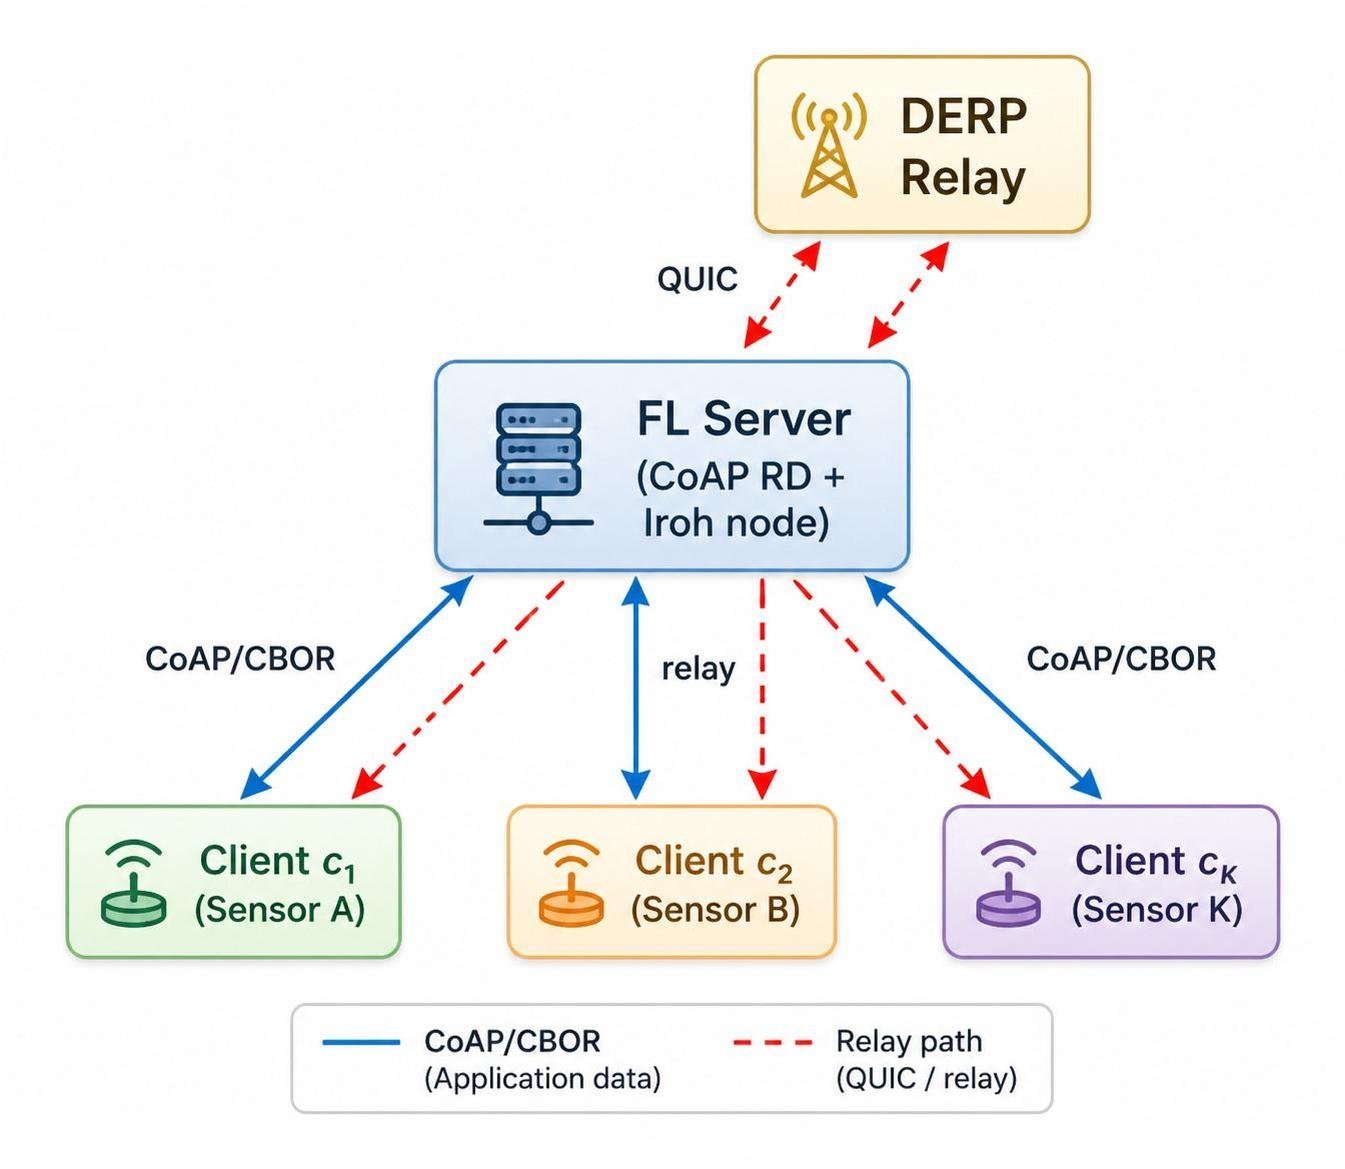
\includegraphics[width=\columnwidth]{FL-Iroh-arch.jpg}
\caption{FL-Iroh architecture. The FL server (CoAP resource directory + Iroh node) coordinates $K$ sensor clients: solid blue arrows are the control plane (registration, discovery, round signaling and application metadata), while dashed red arrows are the Iroh/QUIC relay path through the DERP relay, used transparently for tensor data whenever a direct hole-punched path cannot be validated.}
\label{fig:architecture}
\end{figure}

\begin{figure}[t]
\centering
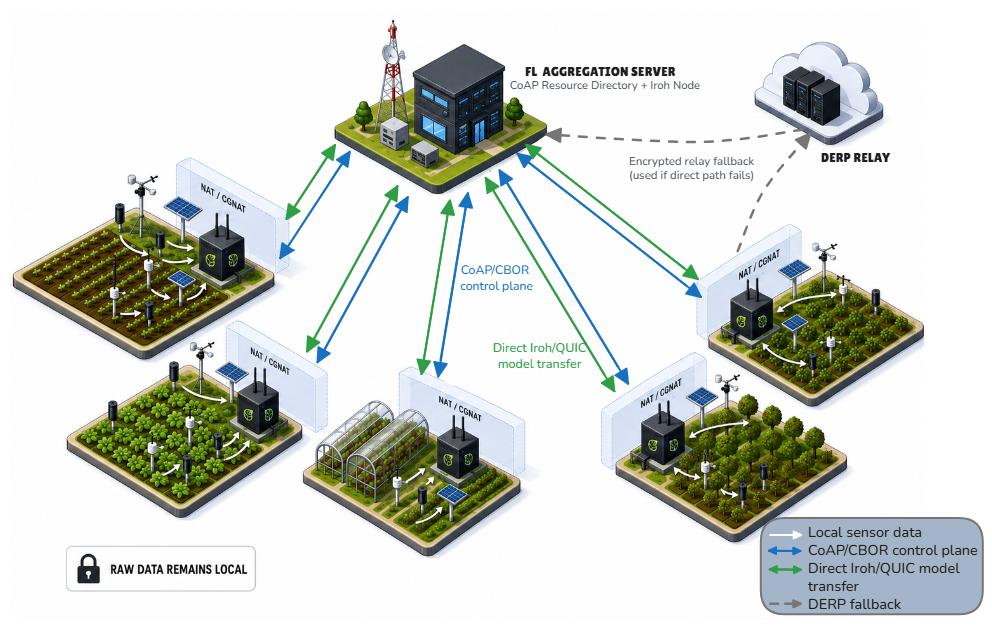
\includegraphics[width=\columnwidth]{physical-deploy.png}
\caption{Target deployment of FL-Iroh in agricultural IoT. Field sensors collect agronomic and meteorological measurements that remain within each farm and are processed by a local FL client behind NAT or CGNAT. Clients register with the aggregator, which admits only allow-listed public keys, and exchange global models and local updates over end-to-end-encrypted Iroh/QUIC connections. If a direct hole-punched path cannot be validated, the encrypted traffic is transparently forwarded through the DERP relay.}
\label{fig:agro}
\end{figure}

\subsection{Node Identity and Admission Control}
\label{sec:admission}

Every node owns a persistent 32-byte Ed25519 secret key; its public key is the node ID used to address it. The QUIC/TLS~1.3 handshake proves possession of the secret key, so a peer cannot claim a node ID it does not own. The aggregator keeps an allow-list of authorized client node IDs (one line per member, distributed out of band when a farm joins the federation). Admission is enforced at three points: (i)~on every incoming Iroh connection, \emph{before} any stream is read, the authenticated remote node ID is checked and unknown peers are closed with an application error code; (ii)~registration (CoAP \texttt{/fl/register}, \texttt{/rd}, or \texttt{fl-ctrl/1}) is refused for node IDs outside the allow-list, and over \texttt{fl-ctrl/1} the registered endpoint must belong to the authenticated sender; (iii)~each round, the aggregator accepts at most one update per \emph{selected} node ID, discarding updates from unselected peers and duplicates. Registering an allow-listed node ID one does not own over CoAP gains nothing: models are addressed to that node ID and updates are only accepted from the peer holding its key.

\subsection{Iroh Transport and Path Selection}
\label{sec:transport}

Iroh~\cite{iroh2024} creates a QUIC endpoint whose \emph{node address} consists of the node ID, a list of candidate direct UDP addresses (local interfaces plus the public mapping discovered via STUN-like probing), and a DERP relay URL. When a node dials another, Iroh (i)~uses the relay for signaling and, immediately, for data; (ii)~probes the candidate direct addresses (hole punching); and (iii)~migrates the QUIC session to a direct path once a probe round trip validates it. Iroh reports the resulting path as \emph{direct} (a validated UDP path), \emph{mixed} (the relay carries traffic while a direct candidate is still being validated) or \emph{relay}. FL-Iroh records this state for every transfer, together with the active address, and we count only \emph{direct} as a hole-punched path; \emph{mixed} transfers are relay-carried.

Two mechanisms harden the transport for unattended operation. \emph{Transfer-level retry}: if a stream is interrupted before the receiver acknowledges it (measured on a 4G CGNAT path in \S\ref{sec:e8}), the sender reopens the connection---letting Iroh re-select a path---and resends, up to a configurable number of attempts; rejections by the peer's allow-list are not retried. \emph{Endpoint watchdog}: after a configurable number of consecutive failed transfers the Iroh endpoint is restarted with the same secret key, so the node ID and pending receivers are preserved. We added the watchdog after observing in hardware tests that, after successive network switches, the endpoint of the Iroh version we use could stop establishing connections until restarted (\S\ref{sec:e8}).

FL-Iroh uses ALPN-based multiplexing: model push, update upload and control messages share a single Iroh endpoint without port allocation, and each ALPN has its own receive queue so that concurrent consumers never block each other.

\subsection{Wire Format}
\label{sec:wire}

Each QUIC unidirectional stream carries one payload:
\begin{equation}
\underbrace{[4\,\text{B}]}_{\text{len}} \;\; \underbrace{[\text{payload}]}_{\text{serialized parameters}} \;\; \underbrace{[32\,\text{B}]}_{\text{SHA-256}}
\label{eq:wire}
\end{equation}
The SHA-256 suffix in Eq.~\eqref{eq:wire} provides integrity verification at the application layer, independent of QUIC's own authentication. The sender waits until the receiver has read the stream to completion before releasing the connection. The framing itself is language-neutral; the prototype serializes PyTorch \texttt{state\_dict} objects with \texttt{torch.save}, and control messages as JSON (\S\ref{sec:agnostic}).

\subsection{CoAP Control Plane and Resource Directory}
\label{sec:coap}

Every node exposes CoAP resources following the CoRE link format~\cite{rfc6690}: \texttt{/fl/capabilities} (hardware, energy state and capability tags such as sensor types, crop or region), \texttt{/iroh/endpoint}, \texttt{/fl/round}, \texttt{/fl/policy}, \texttt{/fl/metrics}, and \texttt{/fl/register} on the aggregator. Responses are JSON or CBOR~\cite{rfc8949}, negotiated with the CoAP Accept option.

Discovery can be performed in two ways. In \emph{probe} mode the aggregator queries \texttt{/fl/capabilities} of every known node and filters client-side, costing one request per node. In \emph{resource-directory} mode, following RFC~9176~\cite{rfc9176}, each node registers once (POST \texttt{/rd} with its tags, role, energy state, lifetime and Iroh endpoint) and the aggregator answers a single lookup, e.g.\ GET \texttt{/rd-lookup/ep} with query \texttt{tag=agri,r3,soil\_moisture} and \texttt{min\_energy=20}, with server-side filtering on any combination of capability tags, role and energy level, optionally paged. Registrations expire after their lifetime unless refreshed. E5 compares both modes up to 5{,}000 endpoints.

\subsection{Round Protocol}
\label{sec:round}

Fig.~\ref{fig:sequence} shows the message sequence of one round and Table~\ref{alg:round} the aggregator's logic (Algorithm~1). A client that misses a round (e.g., while disconnected) simply receives the next global model when it is selected again; late registrations are included from the next round on.

\begin{figure}[t]
\centering
\resizebox{\columnwidth}{!}{%
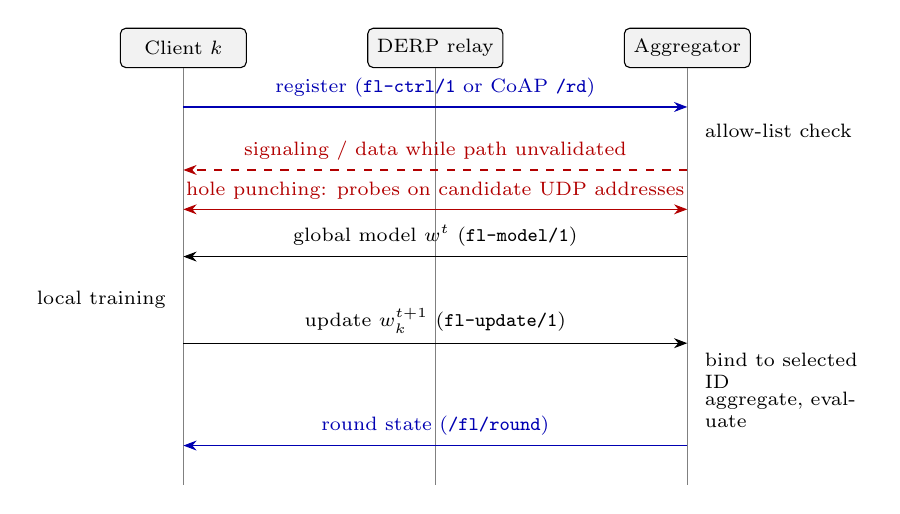
\begin{tikzpicture}[font=\scriptsize, >=Stealth,
  actor/.style={draw, rounded corners=2pt, fill=gray!10, minimum width=1.6cm, minimum height=0.5cm, align=center}]
\node[actor] (c) at (0,0) {Client $k$};
\node[actor] (r) at (3.2,0) {DERP relay};
\node[actor] (s) at (6.4,0) {Aggregator};
\foreach \n in {c,r,s} { \draw[gray] (\n.south) -- ++(0,-5.3); }
\draw[->, blue!70!black] (0,-0.75) -- node[above, pos=0.5] {register (\texttt{fl-ctrl/1} or CoAP \texttt{/rd})} (6.4,-0.75);
\node[anchor=west, align=left, text width=2.0cm] at (6.5,-1.05) {allow-list check};
\draw[->, red!70!black, dashed] (6.4,-1.55) -- node[above] {signaling / data while path unvalidated} (0,-1.55);
\draw[<->, red!70!black] (0,-2.05) -- node[above] {hole punching: probes on candidate UDP addresses} (6.4,-2.05);
\draw[->] (6.4,-2.65) -- node[above] {global model $w^{t}$ (\texttt{fl-model/1})} (0,-2.65);
\node[anchor=east, align=right] at (-0.1,-3.2) {local training};
\draw[->] (0,-3.75) -- node[above] {update $w_k^{t+1}$ (\texttt{fl-update/1})} (6.4,-3.75);
\node[anchor=west, align=left, text width=2.0cm] at (6.5,-4.1) {bind to selected ID};
\node[anchor=west, align=left, text width=2.0cm] at (6.5,-4.6) {aggregate, evaluate};
\draw[->, blue!70!black] (6.4,-5.05) -- node[above] {round state (\texttt{/fl/round})} (0,-5.05);
\end{tikzpicture}}
\caption{Message sequence of one FL-Iroh round. Model and update streams use a validated direct path when one exists and the end-to-end-encrypted relay otherwise; the application code is identical in both cases.}
\label{fig:sequence}
\end{figure}

\begin{table}[t]
\centering
\caption{Algorithm~1: aggregator round $t$ (FL-Iroh server)}
\label{alg:round}
\scriptsize
\begin{tabular}{@{}r p{7.3cm}@{}}
\toprule
1 & $S_t \leftarrow$ select clients among the admitted, registered node IDs (fraction $C$, at least $m$); \\
2 & \textbf{for} $k \in S_t$ \textbf{in parallel}: send $w^{t}$ to node ID $k$ over \texttt{fl-model/1} (retry; drop $k$ on failure); \\
3 & \textbf{if} fewer than $m$ sends succeeded \textbf{then} mark round failed and \textbf{return}; \\
4 & $U \leftarrow \emptyset$; \textbf{until} every sent $k$ answered or timeout $T$: receive $(u, \mathit{id})$ on \texttt{fl-update/1}; \\
5 & \quad \textbf{if} $\mathit{id} \in S_t$ and $\mathit{id}$ not yet in $U$ \textbf{then} $U \leftarrow U \cup \{(\mathit{id}, u)\}$ \textbf{else} discard; \\
6 & $w^{t+1} \leftarrow \texttt{aggregator\_fn}(U)$ \quad (FedAvg, FedGAM, \dots); \\
7 & evaluate $w^{t+1}$; publish round state and model descriptor on CoAP; log per-transfer path and bytes. \\
\bottomrule
\end{tabular}
\end{table}

\subsection{Application Models}

\textbf{AgriMLP} (Crop Recommendation). A four-layer MLP $7 \to 64 \to 64 \to 32 \to 22$ with Batch Normalization and Dropout (rate~0.2) on the first two hidden layers; 7{,}734 trainable parameters ($\approx$32~KB serialized). Inputs are z-score normalized soil macro-nutrients (N, P, K), temperature, humidity, pH, and rainfall.

\textbf{AirMLP} (7-Day-Ahead ICA Forecasting, Outdoor). A four-layer network $6 \to 32 \to 32 \to 16 \to 3$ (1{,}987 parameters, $\approx$14~KB serialized) with the same regularization scheme. Inputs are daily outdoor measurements at time~$t$ (NO$_2$, O$_3$, particulate matter, CO) fused with AEMET meteorological predictors (wind speed, precipitation); the target is the ICA class at $t{+}7$ (\S\ref{sec:e6}).

\textbf{ProphetWrapper} (Federated GAM case study). We wrap Facebook Prophet~\cite{taylor2018prophet} in an \texttt{nn.Module} adapter that exposes the Fourier seasonality coefficients (annual: $N{=}10$ sin/cos pairs; weekly: $N{=}3$) and the wind-speed regressor weight as tensors. Under \textbf{FedGAM} only these shared seasonal terms are averaged (weighted by sample count), while each zone keeps its locally fitted trend ($k$, $m$, $\delta$); under FedAvg all parameters are averaged. Formally, with $\theta_k = (\theta_k^{s}, \theta_k^{\tau})$ the seasonal and trend parameters of zone $k$ and $n_k$ its sample count,
\begin{equation}
\theta^{s} \leftarrow \sum_k \frac{n_k}{\sum_j n_j}\,\theta_k^{s}, \qquad \theta_k^{\tau} \text{ kept local}.
\label{eq:fedgam}
\end{equation}

% =========================================================================
\section{Experimental Evaluation}
\label{sec:evaluation}

We report eleven experiments (Table~\ref{tab:explist}) followed by an operational comparison with Flower-over-Tailscale (\S\ref{sec:flower}). Throughout, we distinguish three connectivity outcomes for every transfer or connection attempt: \emph{direct} (carried over a validated hole-punched UDP path), \emph{relay-carried} (Iroh state \emph{relay} or \emph{mixed}, i.e., the DERP relay carries the traffic while no direct path is validated), and \emph{failed}.

\begin{table}[t]
\centering
\caption{Experiments, research questions and reviewer-requested additions in this revision}
\label{tab:explist}
\scriptsize
\setlength{\tabcolsep}{2.5pt}
\begin{tabular}{@{}l p{4.1cm} l l@{}}
\toprule
\textbf{Exp.} & \textbf{Question} & \textbf{Platform} & \textbf{Transport} \\
\midrule
E1 & Transport throughput (relay path) & PC, RPi & real Iroh \\
E2 & Convergence under non-IID data & HPC & in-process \\
E3 & Connection establishment across classified NATs & PC, RPi & real Iroh \\
E4 & Robustness to client dropout (simulated) & HPC & in-process \\
E5 & CoAP discovery scaling to 5{,}000 endpoints & PC & CoAP \\
E6 & Air-quality forecasting, imbalance-aware metrics & HPC, PC & real Iroh \\
E7 & Operational comparison with Flower + Tailscale (\S\ref{sec:flower}) & HPC & in-process \\
E8 & Forced relay, outages, network switches & RPi, PC & real Iroh \\
E9 & Loss / latency / bandwidth sweep & PC (netem) & real Iroh \\
E10 & Public-key admission control & PC, RPi & real Iroh \\
E11 & Full federation over WAN; RPi resources & RPi, PC & real Iroh \\
\bottomrule
\end{tabular}
\end{table}

\subsection{Experimental Setup}
\label{sec:setup}

\textbf{Hardware.} The edge client is a Raspberry Pi~3 Model~B (quad-core Cortex-A53 at 1.2~GHz, 1~GB RAM; Raspberry Pi OS based on Debian~13, Python~3.13, PyTorch~2.12 CPU build). The aggregator is a laptop PC running the server inside WSL2 (Ubuntu) on Windows~11. Learning-dynamics experiments (E2, E4 and the multi-seed part of E6) run on a single-node HPC cluster (Intel Xeon, 16 cores, no GPU). All experiments use the Iroh~0.35 Python bindings and the public n0 DERP relays.

\textbf{Networks.} Table~\ref{tab:networks} lists the networks used in the hardware experiments. For the networks added in this revision we measured NAT mapping and filtering behavior with RFC~4787/RFC~5780 STUN probes from the device itself (\texttt{scripts/nat\_classify.py} in the artifact): mapping is classified by querying five STUN servers on different IPs from one local UDP port, and filtering by RFC~5780 CHANGE-REQUEST tests. The earlier cross-ISP campaign (PC~$\leftrightarrow$~Raspberry Pi, 300~km apart) used router/ISP configurations that were labeled but not probed; we keep those labels as descriptions of the configured topology.

\begin{table}[t]
\centering
\caption{Networks used in the hardware experiments (RFC~4787 behavior measured with STUN probes; EIM = endpoint-independent mapping; ADF = address-dependent filtering)}
\label{tab:networks}
\scriptsize
\setlength{\tabcolsep}{2.5pt}
\begin{tabular}{@{}l p{3.0cm} l l l@{}}
\toprule
\textbf{Id} & \textbf{Network} & \textbf{Mapping} & \textbf{Filtering} & \textbf{Port pres.} \\
\midrule
N1 & Office Wi-Fi (enterprise NAT) & EIM & ADF & yes \\
N2 & Mobile 4G (Lowi/Vodafone) via phone hotspot: hotspot NAT + carrier NAT & EIM & ADF & no \\
N3 & Home fixed broadband (host OS) & EIM & ADF & yes \\
N3$'$ & N3 seen from WSL2 (additional host NAT) & EIM & ADF & no \\
\midrule
C1--C5 & Earlier cross-ISP campaign: base, ``full-cone'', ``symmetric'', CGNAT (mobile carrier), port-443 firewall & \multicolumn{3}{l}{configured, not probed} \\
\bottomrule
\end{tabular}
\end{table}

\textbf{Software and data.} FL experiments use $K{=}10$ clients unless stated, FedAvg (or FedGAM for the Prophet case study), $E{=}1$ local epoch, SGD (lr$=$0.01, momentum 0.9, weight decay $10^{-4}$), and $R{=}100$ rounds for E2 and E4, $R{=}50$ for E6, $R{=}20$ for E9 and $R{=}30$ for E11. E2 uses SimpleCNN (three Conv--BN--ReLU blocks of 32/64/128 channels, global average pooling and a linear head; 94{,}762 parameters) on CIFAR-10~\cite{cifar2009}. The Crop Recommendation dataset~\cite{cropdataset} contains 2{,}200 records across 22 classes, partitioned IID or with Dirichlet $\alpha \in \{0.1, 0.5, 1.0\}$. The E6 air-quality dataset covers 10 Castilla y Le\'on monitoring zones over 2011--2019 (train: 2011--2018, test: 2019) with a geographic partition (one client per zone) and an IID baseline. Multi-seed runs use a fixed seed registry ($n{=}5$); 95\% confidence intervals use the Student-$t$ distribution.

\textbf{Transport in each experiment.} E2 and E4 study learning dynamics (non-IID data, partial participation) and were run with an in-process loopback transport that delivers the same serialized payloads without the network stack; we report them as statistical experiments and evaluate all transport behavior on real Iroh connections in E1, E3, E6 and E8--E11. Code, per-run results and analysis scripts are available at the anonymized project repository (URL withheld for double-blind review).

\subsection{E1: Transport Throughput}
\label{sec:e1}

We benchmark three transport configurations across four payload sizes (100~KB, 1~MB, 10~MB, 100~MB):

\begin{itemize}
    \item \textbf{HTTP/2 (loopback)}: aiohttp server+client on localhost, serving as a ceiling baseline.
    \item \textbf{iroh\_relay\_loopback}: two in-process Iroh nodes on the same machine, using the public DERP relay \texttt{euw1-1.relay.iroh.network}.
    \item \textbf{iroh\_relay\_wan}: PC as server and the Raspberry Pi (300~km away, different ISP) as client, using the same public DERP relay.
\end{itemize}

Results are shown in Table~\ref{tab:e1}. HTTP/2 peaks at 573~Mbps for 1~MB payloads on loopback, dropping to 244~Mbps at 100~MB (memory bandwidth limited). The iroh relay loopback achieves 27.2~Mbps at 100~KB ($N{=}14$, preliminary). The WAN relay saturates at 2.8~Mbps independent of payload size ($N{=}30$ per cell), which points to a relay-side ceiling (server capacity or per-connection rate limiting on the public relay) rather than QUIC overhead; we did not benchmark a self-hosted relay to separate the two. In E8 the relay delivered 1~MB updates at a median 1.85~Mbps over a 4G uplink, essentially the same as the direct path on that link (1.88~Mbps), so on mobile links the access network rather than the relay was the bottleneck. For AgriMLP and AirMLP updates (14--32~KB) relay transport time is a few hundred milliseconds per round.

\begin{table}[t]
\centering
\caption{E1: Transport Throughput Summary}
\label{tab:e1}
\scriptsize
\setlength{\tabcolsep}{3.5pt}
\begin{tabular}{l r r r r}
\toprule
\textbf{Transport} & \textbf{Payload} & \textbf{Mean (Mbps)} & \textbf{P95 (Mbps)} & \textbf{N} \\
\midrule
HTTP/2               & 100~KB  & 208.2  & 245.5  & 30 \\
HTTP/2               & 1~MB    & 573.6  & 603.3  & 30 \\
HTTP/2               & 10~MB   & 479.2  & 560.3  & 30 \\
HTTP/2               & 100~MB  & 244.6  & 248.9  & 30 \\
\midrule
iroh relay loopback  & 100~KB  & 27.2   & 29.2   & 14 \\
\midrule
iroh relay WAN       & 100~KB  & 2.26   & 2.43   & 30 \\
iroh relay WAN       & 1~MB    & 2.75   & 2.79   & 30 \\
iroh relay WAN       & 10~MB   & 2.81   & 2.82   & 30 \\
iroh relay WAN       & 100~MB  & 2.81   & 2.83   & 30 \\
\bottomrule
\end{tabular}
\end{table}

\subsection{E2: FL Convergence Under Non-IID Data}
\label{sec:e2}

We evaluate FedAvg convergence on CIFAR-10 with SimpleCNN under IID and non-IID (Dirichlet $\alpha{=}0.1$) partitioning ($K{=}10$, $E{=}1$, $R{=}100$, $n{=}5$ seeds; Table~\ref{tab:e2}).

\begin{table}[t]
\centering
\caption{E2: FL Convergence on CIFAR-10 (SimpleCNN, $K{=}10$, $R{=}100$, $n{=}5$ seeds)}
\label{tab:e2}
\footnotesize
\begin{tabular}{l r r}
\toprule
\textbf{Partition} & \textbf{Test Acc. (final)} & \textbf{95\% CI} \\
\midrule
IID                  & 65.86\% & [65.66\%, 66.06\%] \\
Dirichlet $\alpha{=}0.1$ & 44.18\% & [39.45\%, 48.92\%] \\
\bottomrule
\end{tabular}
\end{table}

Under IID partitioning, SimpleCNN converges to 65.86\% test accuracy with a 95\% CI of $\pm$0.2pp. Severe label skew (Dirichlet $\alpha{=}0.1$) lowers accuracy to 44.18\% with a wider CI ($\pm$4.7pp), consistent with prior work~\cite{li2020federated,scaffold2020}. A single-seed sweep confirms a monotonic trend from IID (65.86\%) through $\alpha{=}1.0$ (63.95\%) and $\alpha{=}0.5$ (62.64\%) to $\alpha{=}0.1$. All runs complete their 100 rounds; each round aggregates 3.87~MB of updates ($K{=}10 \times \approx$0.387~MB).

\subsection{E3: Connection Establishment Across Classified NATs}
\label{sec:e3}

\paragraph{Correction of the path classification.} The original submission counted Iroh's \emph{mixed} state as a direct path. While analysing the forced-relay experiments of this revision (\S\ref{sec:e8}), we found that with all outgoing UDP blocked---so that hole punching is impossible---Iroh reports the connection as \emph{mixed}, not \emph{relay}: it keeps a direct candidate address while the relay carries all traffic. Debug logs of every cold start record, for each candidate address, whether a probe round trip has been measured; in all \emph{mixed} cases no candidate had one, i.e., no direct path had been validated. We therefore re-classified the original campaign with the strict criterion (direct = Iroh reports \emph{direct} with a validated address) and report the corrected figures below. This supersedes the transfer-level table and the ``0\% relay'' statements of the original submission; the per-run logs and the re-classification script are in the artifact.

\paragraph{Cold-start campaign.} Each attempt spawns a fresh process with a new Iroh endpoint and NAT-mapping discovery, sends one payload and records the path after a 5~s settle window; attempts are separated by a 20~s pause ($N{=}30$ per scenario). Table~\ref{tab:e3est} reports the corrected results for the original cross-ISP campaign (C1--C5) and a new campaign from the Raspberry Pi on N1 to the PC on N3$'$.

\begin{table*}[t]
\centering
\caption{E3: cold-start connection establishment ($N{=}30$ independent attempts per scenario; strict path classification). \emph{Connected} = direct + relay-carried. Median est.\ = client-side dial-to-connection time of successful attempts. The C1 base profile ran with a remote client and therefore also traversed the WAN.}
\label{tab:e3est}
\scriptsize
\setlength{\tabcolsep}{4pt}
\begin{tabular}{l l r r r r r r}
\toprule
\textbf{Scenario} & \textbf{Path} & \textbf{Attempts} & \textbf{Direct} & \textbf{Relay-carried} & \textbf{Failed} & \textbf{Connected (\%)} & \textbf{Median est.} \\
\midrule
C1 base profile (over WAN)   & PC $\leftrightarrow$ RPi, 300~km & 30 & 25 & 4  & 1 & 96.7  & 415~ms \\
C2 ``full-cone'' NAT         & PC $\leftrightarrow$ RPi, 300~km & 30 & 27 & 2  & 1 & 96.7  & 459~ms \\
C3 ``symmetric'' NAT         & PC $\leftrightarrow$ RPi, 300~km & 30 & 14 & 15 & 1 & 96.7  & 391~ms \\
C4 CGNAT (mobile carrier)    & PC $\leftrightarrow$ RPi, 300~km & 30 & 23 & 4  & 3 & 90.0  & 439~ms \\
C5 port-443 firewall         & PC $\leftrightarrow$ RPi, 300~km & 30 & 0  & 30 & 0 & 100.0 & 1429~ms \\
\midrule
\textbf{C2--C5 (WAN)}        &                         & 120 & \textbf{64} & \textbf{51} & 5 & \textbf{95.8} & \\
\midrule
N1 $\to$ N3$'$ (new)         & RPi (office) $\to$ PC (home) & 30 & 0 & 30 & 0 & 100.0 & 176~ms \\
\bottomrule
\end{tabular}
\end{table*}

Three observations follow. First, connectivity is robust: 115 of 120 WAN cold starts in the original campaign and 30 of 30 in the new office--home campaign established a working connection, and every failure was a first-attempt timeout without retry. Second, a validated direct path within the 5~s window is far from universal: 64 of 120 (53.3\%) in the original campaign, with the clearest gap under the scenario labeled symmetric NAT (14/30) and none under the port-443 firewall, where UDP was blocked and all 30 connections were relay-carried. Third, in the office--home campaign every cold start began relay-carried: a freshly started node dials before it has discovered its own public mapping, and the receiving side ran behind the extra WSL2 host NAT (N3$'$), which rewrites ports. The same pair of networks yields direct paths immediately once a node is long-lived (60/60 transfers home$\to$office, \S\ref{sec:e8}), which is the relevant regime for FL, where nodes stay up across rounds. Cold-start figures therefore characterize the first seconds of a connection; the steady-state path is characterized in E8.

\subsection{E4: Robustness to Client Dropout (Simulated)}
\label{sec:e4}

We simulate dropout by withholding a random fraction $p \in \{0, 10, 30, 50\}$\% of clients from each round, under IID and Dirichlet $\alpha{=}0.1$ partitions of the Crop Recommendation dataset; FedAvg aggregates whichever updates arrive. This isolates the learning effect of partial participation; real network disconnections, reconnection and rejoining are measured separately on hardware in E8 and E11. Every configuration is replicated over $n{=}5$ seeds (Table~\ref{tab:e4}).

\begin{table*}[t]
\centering
\caption{E4: Robustness to simulated dropout (Crop Recommendation, AgriMLP, $K{=}10$, $R{=}100$, $n{=}5$ seeds; accuracy as mean $\pm$ half-width of the 95\% CI, in pp). Rounds$\to$40\% is the median across seeds of the first round exceeding 40\% test accuracy. A centralized reference ($K{=}1$, full training set, same loop and seeds) reaches 97.9\% $\pm$ 0.3.}
\label{tab:e4}
\footnotesize
\begin{tabular}{l l r r r r}
\toprule
\textbf{Partition} & \textbf{Dropout} & \textbf{Acc (final)} & \textbf{Acc (peak)} & \textbf{Rounds$\to$40\%} & \textbf{Completed} \\
\midrule
IID & 0\%  & 87.3\% $\pm$ 2.0 & 87.6\% $\pm$ 1.7 & 23 & 100/100 \\
IID & 10\% & 86.5\% $\pm$ 3.4 & 87.4\% $\pm$ 2.8 & 22 & 100/100 \\
IID & 30\% & 86.2\% $\pm$ 3.3 & 88.0\% $\pm$ 2.1 & 22 & 100/100 \\
IID & 50\% & 86.4\% $\pm$ 2.2 & 87.1\% $\pm$ 1.8 & 23 & 100/100 \\
\midrule
Dirichlet $\alpha{=}0.1$ & 0\%  & 71.8\% $\pm$ 5.4 & 72.0\% $\pm$ 5.5 & 33 & 100/100 \\
Dirichlet $\alpha{=}0.1$ & 10\% & 70.7\% $\pm$ 2.5 & 72.4\% $\pm$ 5.0 & 34 & 100/100 \\
Dirichlet $\alpha{=}0.1$ & 30\% & 71.1\% $\pm$ 8.1 & 73.9\% $\pm$ 5.9 & 35 & 100/100 \\
Dirichlet $\alpha{=}0.1$ & 50\% & 67.9\% $\pm$ 6.8 & 69.7\% $\pm$ 5.6 & 37 & 100/100 \\
\bottomrule
\end{tabular}
\end{table*}

Under IID partitioning, accuracy is statistically flat across dropout rates (86.2--87.3\% final, overlapping CIs). Under Dirichlet $\alpha{=}0.1$, label skew costs roughly 15pp, convergence is slower (median 33--37 rounds to 40\%, vs.\ 22--23 under IID), and 50\% dropout shows the lowest mean (67.9\%); with CIs of $\pm$5--8pp no pairwise difference is resolvable at $n{=}5$. Dropout caused neither divergence nor round failures. The federated IID configurations sit $\approx$11pp below the centralized reference (97.9\%), a gap attributable to federation ($K{=}10$, $E{=}1$) rather than to dropout.

\subsection{E5: CoAP Discovery Scaling}
\label{sec:e5}

We compare the two discovery modes of \S\ref{sec:coap} for $N \in \{10, 100, 500, 1{,}000, 2{,}000, 5{,}000\}$ endpoints. Each endpoint carries a domain tag (\texttt{agri}/\texttt{air}), one of ten region tags and two or three sensor tags; queries with one, two and three tags select about 50\%, 5\% and 1--2\% of the nodes. In \emph{probe} mode every endpoint is a separate CoAP server on its own port (hosted by worker processes on one machine, up to $N{=}1{,}000$); in \emph{RD} mode the aggregator runs in a separate process and all endpoints first register concurrently (up to 64 registrations in flight). Wire bytes are the encoded CoAP messages in both directions. Results are medians over 30 lookups (10 for probe) on loopback, so they measure processing and protocol cost; on a WAN, probe cost grows with the RTT of each request, whereas an RD lookup is a single exchange.

\begin{table}[t]
\centering
\caption{E5: discovery latency and wire bytes (median; loopback). Probe = one query per endpoint with client-side filtering; RD = one lookup with server-side filtering.}
\label{tab:e5}
\scriptsize
\setlength{\tabcolsep}{2.5pt}
\begin{tabular}{@{}r l r r r r@{}}
\toprule
\textbf{N} & \textbf{Mode} & \textbf{Tags} & \textbf{Match} & \textbf{ms} & \textbf{Bytes} \\
\midrule
100   & probe & 3 & 1    & 57.0   & 45{,}927 \\
100   & RD    & 3 & 1    & 1.5    & 336 \\
1{,}000 & probe & 1 & 500 & 978.0  & 583{,}649 \\
1{,}000 & probe & 3 & 11  & 795.9  & 459{,}790 \\
1{,}000 & RD    & 1 & 500 & 92.8   & 137{,}519 \\
1{,}000 & RD    & 3 & 11  & 3.1    & 3{,}156 \\
5{,}000 & RD    & 1 & 2{,}500 & 873.7 & 692{,}651 \\
5{,}000 & RD    & 2 & 222 & 66.8   & 61{,}633 \\
5{,}000 & RD    & 3 & 68  & 18.9   & 19{,}626 \\
\midrule
\multicolumn{6}{@{}l}{RD registration, $N{=}5{,}000$: all registered; median 220~ms, p95 329~ms} \\
\bottomrule
\end{tabular}
\end{table}

Probe discovery grows linearly with the number of endpoints regardless of how many match (0.8--1.0~s and 460--580~KB at 1{,}000 nodes), because every node must be queried. With the resource directory, cost scales with the number of \emph{matching} endpoints: a three-tag query over 5{,}000 registered endpoints takes 18.9~ms and 19.6~KB, and paging (\texttt{count}, \texttt{page}) bounds the response size of broad queries. Concurrent registration of all 5{,}000 endpoints completed without failures (median per-registration latency 220~ms with up to 64 in flight). This replaces the original E5, whose loop queried a single server repeatedly and extrapolated byte counts; the corrected probe numbers at 100 nodes (57--97~ms) are of the same order as originally reported.

\subsection{E6: Air Quality Federated Learning}
\label{sec:e6}

\textbf{Dataset and task.} We use the Castilla y Le\'on daily air quality archive~\cite{cyl2023airquality} (10 monitoring zones) merged with AEMET~\cite{aemet2023} meteorological data (wind speed, precipitation), restricted to 2011--2019 to avoid the COVID-19 lockdown artifact~\cite{lopezblanco2024airquality}. The task is 7-day-ahead ICA forecasting: given outdoor readings at day~$t$, predict the ICA class at $t{+}7$. Labels use training-set NO$_2$ terciles ($T_1{=}7.5$, $T_2{=}13.0~\mu$g/m$^3$), balanced in-sample (\textit{Bajo}, \textit{Medio}, \textit{Alto}); because NO$_2$ declined over the decade, the 2019 test year is imbalanced (49.3\% \textit{Bajo}, 27.8\% \textit{Medio}, 22.9\% \textit{Alto}). We therefore report, besides accuracy, macro-F1, balanced accuracy, per-class recall and the confusion matrix (Table~\ref{tab:e6}).

\textbf{Configurations.} AirMLP and AirLSTM (a 7-day input window) with FedAvg under geographic and IID partitions, and ProphetWrapper with FedAvg or FedGAM; $n{=}5$ seeds, $R{=}50$, real Iroh transport. Prophet models are evaluated per zone: each zone's model (federated seasonality plus its local trend under FedGAM; retrained from the full global state under FedAvg) predicts its own test year, and predictions are pooled across zones.

\begin{table*}[t]
\centering
\caption{E6: 7-day-ahead ICA forecasting on the 2019 test year ($K{=}10$, $R{=}50$, $n{=}5$ seeds; mean $\pm$ half-width of the 95\% CI, in \%; real Iroh transport). Class distribution 49.3/27.8/22.9\% (\textit{Bajo/Medio/Alto}).}
\label{tab:e6}
\scriptsize
\setlength{\tabcolsep}{4pt}
\begin{tabular}{l l r r r r r r}
\toprule
\textbf{Model} & \textbf{Partition} & \textbf{Accuracy} & \textbf{Balanced acc.} & \textbf{Macro-F1} & \textbf{Recall \textit{Bajo}} & \textbf{Recall \textit{Medio}} & \textbf{Recall \textit{Alto}} \\
\midrule
Majority class (train)          & ---        & 22.94\% & 33.33\% & 12.44\% & 0.0\% & 0.0\% & 100.0\% \\
Persistence ($t{-}7$)           & ---        & 47.54\% & 43.07\% & 43.13\% & 62.2\% & 30.7\% & 36.3\% \\
\midrule
AirMLP (FedAvg)                 & Geographic & 46.85 $\pm$ 1.02 & 42.22 $\pm$ 0.48 & 40.25 $\pm$ 0.23 & 64.8 $\pm$ 3.7 & 15.3 $\pm$ 2.6 & 46.6 $\pm$ 3.6 \\
AirMLP (FedAvg)                 & IID        & 49.64 $\pm$ 0.61 & 44.93 $\pm$ 0.61 & 43.05 $\pm$ 0.93 & 68.0 $\pm$ 2.0 & 17.2 $\pm$ 2.4 & 49.6 $\pm$ 1.8 \\
AirLSTM (FedAvg)                & Geographic & 53.17 $\pm$ 0.55 & 48.77 $\pm$ 0.42 & 48.11 $\pm$ 0.52 & 69.6 $\pm$ 3.2 & 27.8 $\pm$ 2.9 & 48.9 $\pm$ 2.0 \\
AirLSTM (FedAvg)                & IID        & 55.00 $\pm$ 0.31 & 49.44 $\pm$ 0.34 & 49.07 $\pm$ 0.58 & 74.8 $\pm$ 0.7 & 28.0 $\pm$ 2.5 & 45.6 $\pm$ 1.4 \\
\midrule
ProphetWrapper (FedAvg)         & Geographic & 56.44$^{\ddagger}$ & 48.70 & 49.42 & 79.0 & 36.4 & 30.6 \\
ProphetWrapper (FedAvg)         & IID$^{\S}$ & 57.58 $\pm$ 0.33 & 42.85 $\pm$ 0.35 & 35.63 $\pm$ 0.48 & 63.4 $\pm$ 0.6 & 64.4 $\pm$ 1.2 & 0.8 $\pm$ 0.7 \\
ProphetWrapper (FedGAM)         & Geographic & 56.78$^{\ddagger}$ & 49.18 & 49.94 & 78.9 & 37.5 & 31.1 \\
ProphetWrapper (FedGAM)         & IID$^{\S}$ & 57.93 $\pm$ 0.52 & 42.93 $\pm$ 0.34 & 35.77 $\pm$ 0.47 & 63.9 $\pm$ 0.8 & 64.2 $\pm$ 1.0 & 0.8 $\pm$ 0.7 \\
\bottomrule
\end{tabular}
\vspace{0.3em}

{\scriptsize $^{\ddagger}$Prophet geographic runs are deterministic MAP fits: all five seeds coincide (no CI). $^{\S}$Evaluated on the 2019 test year of a single zone (inherited from the original evaluation code), whose class distribution differs; not comparable with the other rows.}
\end{table*}

\begin{table}[t]
\centering
\caption{E6: confusion matrices summed over five seeds, row-normalized (\%; rows = true class, columns = predicted \textit{Bajo/Medio/Alto})}
\label{tab:e6cm}
\scriptsize
\setlength{\tabcolsep}{3pt}
\begin{tabular}{@{}l l r r r@{}}
\toprule
\textbf{Model (IID)} & \textbf{True} & \textbf{Bajo} & \textbf{Medio} & \textbf{Alto} \\
\midrule
AirMLP  & \textit{Bajo}  & 68.0 & 10.9 & 21.1 \\
        & \textit{Medio} & 47.0 & 17.2 & 35.8 \\
        & \textit{Alto}  & 34.0 & 16.4 & 49.6 \\
\midrule
AirLSTM & \textit{Bajo}  & 74.8 & 14.3 & 10.9 \\
        & \textit{Medio} & 44.5 & 28.0 & 27.6 \\
        & \textit{Alto}  & 28.4 & 26.0 & 45.6 \\
\bottomrule
\end{tabular}
\end{table}

\textbf{Imbalance-aware results.} Accuracy alone overstates the difficulty gap between models and hides how they fail. The 7-day persistence forecaster reaches 47.5\% accuracy but only 43.1\% macro-F1 and balanced accuracy. The memoryless AirMLP does not beat it on the imbalance-aware metrics (macro-F1 40.3\% geographic, 43.1\% IID): it mainly separates the extreme classes and almost never predicts \textit{Medio} correctly (recall 15--17\%), which it confuses with both neighbors (Table~\ref{tab:e6cm}). AirLSTM, which sees a 7-day input window, improves every metric over persistence by about 5--6pp (macro-F1 48.1\% geographic, 49.1\% IID; balanced accuracy 48.8--49.4\%) and nearly doubles the recall of \textit{Medio} (28\%), which remains the hardest class for all models because it is a narrow band between two terciles. The geographic (non-IID) partition costs 1--3pp on every metric for both neural models. The accuracy of AirMLP over real Iroh connections (46.9\% and 49.6\%) matches the values obtained with the in-process transport in the original submission (47.3\% and 49.6\%), a further check that the transport does not alter learning outcomes. The federated Prophet model evaluated over all ten zones (geographic partition) reaches 49.4--49.9\% macro-F1 and 48.7--49.2\% balanced accuracy, on par with AirLSTM and about 6.5pp above persistence; its higher accuracy (56.4--56.8\%) comes largely from the majority class (recall of \textit{Bajo} 79\%, of \textit{Alto} 31\%). The imbalance-aware metrics also exposed a flaw in our original evaluation: in the IID configuration the Prophet models were scored on the test year of a single zone only. On that zone they almost never predict \textit{Alto} (recall below 1\%) and reach only 35.6--35.8\% macro-F1, so the 57.9\% accuracy reported for Prophet-IID in the original submission is not comparable with the other configurations and should not be read as an improvement over persistence. We keep these rows for transparency and base all comparisons on the geographic runs.

\textbf{FedGAM case study.} Switching from FedAvg to FedGAM requires a single server-side change (\texttt{aggregator\_fn}); the same Iroh channels carry AirMLP tensors (1{,}987 parameters) and Prophet Fourier coefficients (27 parameters). Prophet+FedGAM and Prophet+FedAvg are practically indistinguishable (geographic: 49.94\% vs.\ 49.42\% macro-F1, 49.18\% vs.\ 48.70\% balanced accuracy; IID: 35.77\% vs.\ 35.63\% macro-F1). We also tested the regime in which partial aggregation might matter most, with only one year of local history per zone: both rules then fail on this task (geographic macro-F1 18.5\% with FedGAM and 16.7\% with FedAvg, predicting mostly \textit{Alto}), so partial aggregation does not rescue short histories here either. With eight years of local history each zone can estimate its own trend, so restricting aggregation to the seasonal terms brings no measurable benefit here; FedGAM is therefore presented as an example of a model-specific aggregation rule deployed without transport changes, not as a performance contribution.

\subsection{E8: Forced Relay, Outages and Network Switches}
\label{sec:e8}

E8 exercises the relay and the recovery paths on real hardware. A long-lived client on the Raspberry Pi sends a 1~MB update every 5~s to a long-lived server; every transfer re-dials the server by node ID, as the FL data plane does, and the path, active address, retries and local IP addresses are logged per transfer. Perturbations are injected on the Raspberry Pi: blocking all outgoing UDP except DNS with an nftables rule (hole punching becomes impossible and only the relay, which uses HTTPS over TCP, remains), taking the Wi-Fi interface down, and switching between networks with NetworkManager. Throughout E8--E11 a second nftables rule prevents Iroh from using the Tailscale overlay addresses present on the test devices, so that a ``direct'' path is always an Iroh hole-punched path; every transfer is additionally audited for overlay addresses.

\begin{table*}[t]
\centering
\caption{E8: delivery and path per phase (Raspberry Pi on N2 mobile CGNAT $\to$ PC on N1; 1~MB every 5~s; medians)}
\label{tab:e8}
\scriptsize
\setlength{\tabcolsep}{6pt}
\begin{tabular}{@{}l r r r r r@{}}
\toprule
\textbf{Phase} & \textbf{Sent} & \textbf{Delivered} & \textbf{Direct} & \textbf{Relay-carried} & \textbf{Goodput (Mbps)} \\
\midrule
UDP open, start              & 57  & 54 (94.7\%)  & 53  & 1   & \multirow{3}{*}{1.88} \\
UDP open, after unblock 1    & 55  & 40 (72.7\%)  & 39  & 1   & \\
UDP open, after unblock 2    & 57  & 46 (80.7\%)  & 46  & 0   & \\
UDP blocked (2 windows)      & 190 & 190 (100\%)  & 2$^{*}$ & 188 & 1.85 \\
\midrule
\multicolumn{6}{@{}l}{Fallback to relay after blocking: first delivery after 28.1~s and 28.4~s, no transfer lost} \\
\multicolumn{6}{@{}l}{Return to direct after unblocking: 1.9~s and 3.8~s} \\
\bottomrule
\end{tabular}
\vspace{0.3em}

{\scriptsize $^{*}$Classified at the moment of unblocking; one carried a Tailscale address and is excluded from direct counts.}
\end{table*}

\textbf{Forced relay (Table~\ref{tab:e8}).} With UDP blocked, all 190 transfers were delivered over the relay, at the same goodput as the direct path because the 4G uplink, not the relay, was the bottleneck. The switch to the relay took about 28~s, during which the in-flight transfer stalled but was not lost; on unblocking, the path returned to direct within 4~s. On this mobile CGNAT the direct path was less reliable than the relay: 5.3\% of direct transfers were interrupted mid-stream at the start of the run and 19--27\% after the UDP block was lifted, while none of the relay-carried transfers failed. This observation motivated the transfer-level retry of \S\ref{sec:transport}.

\textbf{Outages and network switches.} With transfer retry enabled, a second 30-minute run on N2 delivered 49 of 50 transfers in the first window (two delivered on a retry) and 202 of 213 overall. A 60~s Wi-Fi outage lost no transfer: the in-flight transfer waited and completed, and the first new transfer succeeded 15.6~s after the link came back. During a 120~s outage two transfers timed out, and delivery resumed immediately after the link returned. Switching from 4G to the office Wi-Fi (N2$\to$N1; new local address, new NAT mapping) restored delivery after 4.3~s, now over a direct LAN path to the PC. The opposite switch (N1$\to$N2) did not recover within the remaining five minutes: the Iroh endpoint stopped establishing connections until the process was restarted, even though the 4G link itself was working. We added the endpoint watchdog of \S\ref{sec:transport} as a mitigation (restart with the same key after consecutive failures; covered by the test suite); validating it with repeated network switches in the field remains future work.

\textbf{Long-lived sessions.} Between long-lived nodes the steady-state path is direct: 138 of 140 delivered transfers in the open-UDP phases of the 4G run, and 60 of 60 transfers from the PC on N3$'$ to the Raspberry Pi on N1 (median 266~ms per 64~KB). The exception is a node behind the WSL2 host NAT acting as the \emph{receiver}: in E11 the Raspberry Pi's transfers to and from the aggregator in WSL2 were relay-carried (56 of 58), which we attribute to the additional port-rewriting NAT in front of the server process.

\subsection{E9: Degraded Networks}
\label{sec:e9}

To evaluate behavior on lossy and slow rural links we ran the full FL workload (AirMLP, 10 clients, geographic partition, 20 rounds) and a transfer benchmark (100~KB, 1~MB and 10~MB, 10 transfers each) over real Iroh connections inside an isolated Linux network namespace, applying \texttt{tc-netem} to all traffic: one-way delay of 25--250~ms, jitter, loss of 1--20\%, rate limits of 10~Mbit/s to 512~kbit/s, and two combined profiles. All peers share the impaired link, so a rate limit is shared by concurrent flows. Table~\ref{tab:e9} summarizes the results.

\begin{table*}[t]
\centering
\caption{E9: FL rounds and transfers under emulated network impairments (one-way delay; loss per direction; 20 rounds, 10 clients; medians). Accuracy: final round (best round in parentheses).}
\label{tab:e9}
\footnotesize
\begin{tabular}{l r r r r r r}
\toprule
\textbf{Condition} & \textbf{Rounds OK} & \textbf{Round (s)} & \textbf{Accuracy} & \textbf{Macro-F1} & \textbf{1~MB (s)} & \textbf{10~MB (s)} \\
\midrule
No impairment                          & 20/20 & 1.4  & 46.5\% (47.2) & 38.7\% & 0.13 & 1.2 \\
Delay 25~ms                            & 20/20 & 1.6  & 46.8\% & 39.3\% & 0.60 & 2.2 \\
Delay 100~ms                           & 20/20 & 2.3  & 46.3\% & 38.4\% & 1.86 & 4.6 \\
Delay 250~ms                           & 20/20 & 3.7  & 46.6\% & 38.4\% & 4.37 & 9.5 \\
Delay 100~ms $\pm$ 30~ms               & 20/20 & 2.7  & 46.8\% & 38.1\% & 2.00 & 7.0 \\
Loss 1\%                               & 20/20 & 1.9  & 46.6\% & 40.0\% & 0.15 & 1.5 \\
Loss 5\%                               & 20/20 & 2.5  & 44.3\% & 36.5\% & 0.23 & 1.9 \\
Loss 10\%                              & 20/20 & 3.3  & 48.4\% & 39.1\% & 0.27 & 2.6 \\
Loss 20\%                              & 20/20 & 8.7  & 26.8\% (46.9) & 21.9\% & 1.70 & 10.6 \\
Rate 2~Mbit/s                          & 20/20 & 2.7  & 46.5\% & 38.9\% & 4.49 & 43.8 \\
Rate 512~kbit/s                        & 20/20 & 10.7 & 46.7\% & 38.9\% & 17.0 & 167 \\
Rural LTE (30$\pm$10~ms, 2\%, 5~Mbit/s) & 20/20 & 4.1 & 46.8\% & 38.3\% & 2.14 & 27.2 \\
Harsh rural (75$\pm$25~ms, 10\%, 1~Mbit/s) & 20/20 & 6.5 & 46.6\% & 38.5\% & 26.2 & failed$^{\dagger}$ \\
\bottomrule
\end{tabular}
\vspace{0.3em}

{\scriptsize $^{\dagger}$0/10 transfers of 10~MB completed within the 180~s timeout. A jitter profile that reorders packets (normal-distributed delay without rate shaping) stalled the run and is excluded; reordering of that magnitude is atypical of real links.}
\end{table*}

All 320 rounds of the 16 completed conditions finished successfully (13 conditions are shown). For the 14~KB updates of AirMLP, impairments lengthen rounds (from 1.4~s to 3.7~s at 250~ms delay, 8.7~s at 20\% loss and 10.7~s at 512~kbit/s) but do not change final accuracy or macro-F1, which stay within the seed-to-seed range of the unimpaired run, with one exception: at 20\% loss two rounds aggregated only 8 and 5 of the 10 clients because updates arrived after the round timeout, and the last round was the 5-client one, so its non-IID aggregate drops to 26.8\% (the best round of that run reached 46.9\%). Payload size is what makes QUIC's behavior visible: 10~MB transfers grow from 1.2~s to 9.5~s at 250~ms delay and 167~s at 512~kbit/s, and fail entirely under the harsh rural profile. For edge-sized models the transport is not the limiting factor; for multi-megabyte models on such links, update compression or longer round deadlines would be required.

\subsection{E10: Public-Key Admission Control}
\label{sec:e10}

We measure admission control (\S\ref{sec:admission}) on loopback and over the WAN (aggregator on N3$'$, Raspberry Pi on N1). An authorized client holding an allow-listed key and an unauthorized client with a fresh key each attempt 30 transfers; we also test a peer that registers another node's endpoint over \texttt{fl-ctrl/1} (Table~\ref{tab:e10}).

\begin{table}[t]
\centering
\caption{E10: admission control ($N{=}30$ attempts each; medians)}
\label{tab:e10}
\scriptsize
\setlength{\tabcolsep}{3pt}
\begin{tabular}{@{}l r r@{}}
\toprule
\textbf{Metric} & \textbf{Loopback} & \textbf{WAN (N1$\to$N3$'$)} \\
\midrule
Unauthorized payloads accepted        & 0/30     & 0/30 \\
Unauthorized attempts rejected/logged & 30/30    & 30/30 \\
Time to rejection (client view)       & 10.1~ms  & 329~ms \\
Authorized transfers delivered        & 30/30    & 30/30 \\
Authorized latency, allow-list off/on & 11.0 / 11.1~ms & --- / 3.97~s$^{\ddagger}$ \\
Spoofed registration rejected         & yes      & --- \\
\bottomrule
\end{tabular}
\vspace{0.3em}

{\scriptsize $^{\ddagger}$64~KB, relay-carried (receiver behind the WSL2 host NAT).}
\end{table}

No unauthorized payload was ever accepted, rejection costs one handshake plus one round trip (10~ms on loopback, 0.33~s over the WAN), and the allow-list check adds no measurable latency to authorized transfers. Because the check runs on the authenticated key before any stream is read, an unauthorized peer cannot inject an update; together with the per-round binding of updates to selected node IDs it also prevents a member from submitting several updates per round.

\subsection{E11: Federation over the WAN on a Raspberry Pi~3B}
\label{sec:e11}

Finally, we ran a complete federation across two sites: the aggregator on the PC at home (N3$'$) and three clients registered over \texttt{fl-ctrl/1} by public key---the Raspberry Pi~3B in the office (N1, zone 0) and two clients on the PC (zones 1 and 2)---with the air-quality task, AirMLP, $R{=}30$ and a minimum of two clients per round. No port forwarding, VPN or public IP was configured. The Raspberry Pi recorded CPU time, resident memory and system load per round phase (Table~\ref{tab:e11}). The Raspberry Pi~3B has no power sensor, so energy is estimated with a linear model $P = P_\text{idle} + (P_\text{max}-P_\text{idle})\,u$ on the system CPU utilization $u$, with board-level $P_\text{idle}{=}1.4$~W and $P_\text{max}{=}3.7$~W~\cite{geerlingpower}; these values are estimates, not measurements.

\begin{table}[t]
\centering
\caption{E11: per-round resource use on the Raspberry Pi~3B client (AirMLP, 14~KB updates; medians over 29 rounds; energy estimated)}
\label{tab:e11}
\scriptsize
\setlength{\tabcolsep}{3pt}
\begin{tabular}{@{}l r r r r@{}}
\toprule
\textbf{Phase} & \textbf{Wall (s)} & \textbf{CPU (s)} & \textbf{Power (W)} & \textbf{Energy (J)} \\
\midrule
Receive model (incl.\ waiting) & 3.10 & 0.11 & 1.46 & 4.5 \\
Local training (1 epoch)       & 1.02 & 2.79 & 2.86 & 2.9 \\
Send update                    & 3.45 & 0.20 & 1.51 & 5.2 \\
\midrule
\multicolumn{5}{@{}l}{Resident memory: 255~MB after start-up, 419~MB peak (of 1~GB)} \\
\bottomrule
\end{tabular}
\end{table}

The Raspberry Pi joined the federation shortly after the first round and took part in every subsequent round: 29 of 30 rounds completed, 27 with all three clients, at a median of 7.9~s per round (p95 21.3~s). The last round failed because of a race we found in this experiment: when the receiver closed a connection right after reading a model, the sender sometimes saw the close before the acknowledgement and resent the model, so clients occasionally trained twice per server round and finished early (four stale updates were discarded by the per-round binding of \S\ref{sec:admission}). Receivers now close with an explicit receipt code that senders treat as delivery; with this fix the live comparison of \S\ref{sec:flower}, on the same hardware, completed 30 of 30 rounds with all clients and no discarded update. Local training is cheap on this device---1.0~s of wall time and 2.8~s of CPU time (multi-core) per epoch---while the communication phases are dominated by waiting for other clients and by the relay-carried path to the aggregator in WSL2 (56 of 58 Raspberry Pi transfers; \S\ref{sec:e8}). Memory, not computation, is the tighter constraint: the Python/PyTorch runtime occupies 255--419~MB, about 40\% of the device's RAM, which supports our recommendation of a native client runtime for smaller devices (\S\ref{sec:agnostic}). We also note a deployment pitfall: the default PyPI PyTorch wheel for 64-bit ARM is built for newer ARMv8.2 server cores and terminates with an illegal-instruction error during back-propagation on Cortex-A53/A72 boards; the CPU-only wheel works.

\subsection{Operational Comparison with Flower over Tailscale}
\label{sec:flower}


The closest deployable alternative to FL-Iroh for NAT-constrained FL is to run a conventional framework (Flower~\cite{flower2022}) over a WireGuard mesh VPN such as Tailscale~\cite{tailscale2023}, which gives every node a stable virtual IP and traverses NAT\slash CGNAT through DERP-style relays. Both stacks rely on relay-assisted NAT traversal and end-to-end encryption; the difference is \emph{where} connectivity lives. Table~\ref{tab:e7} contrasts the two along eight operational axes; it is an architectural comparison, complemented by an accuracy-parity check (Table~\ref{tab:e7acc}).

\begin{table*}[t]
\centering
\caption{FL-Iroh vs.\ Flower-over-Tailscale operational comparison}
\label{tab:e7}
\footnotesize
\renewcommand{\arraystretch}{1.25}
\setlength{\tabcolsep}{4pt}
\begin{tabular}{p{2.4cm} p{6.2cm} p{6.2cm}}
\toprule
\textbf{Axis} & \textbf{FL-Iroh} & \textbf{Flower + Tailscale} \\
\midrule
NAT / CGNAT traversal & Built into the application transport: QUIC hole-punching with transparent DERP relay fallback (E2E encrypted) & Delegated to the Tailscale overlay (WireGuard + DERP); Flower itself still needs a reachable server address \\
Server reachability & Peer addressed by 32-byte public node ID; no routable server IP required & Clients must know the server's Tailnet IP (100.x.y.z); centralized star topology \\
Federation membership & Allow-list of public keys enforced by the aggregator at the transport level (E10) & Tailnet membership and ACLs managed in the Tailscale control plane \\
External infrastructure & Public or self-hosted DERP relay only (stateless, swappable) & Tailscale coordination server (control plane) $+$ DERP $+$ long-lived FL server process \\
Extra system daemon & None---userspace library, no elevated privileges & \texttt{tailscaled} system daemon on every node (typically root / \texttt{NET\_ADMIN}) \\
Transport encryption & End-to-end QUIC/TLS~1.3 (relay sees only ciphertext) & End-to-end WireGuard (relay sees only ciphertext) \\
Manual setup per node & Generate key, send node ID to the coordinator, receive the aggregator's endpoint file & Install \texttt{tailscaled}, authenticate node to tailnet, discover server IP \\
Account / ToS dependency & No account; default public relay operated by n0 (subject to its terms), fully self-hostable & Tailscale account $+$ ACL policy management (free-tier device/user caps) \\
\bottomrule
\end{tabular}
\end{table*}

\paragraph{Accuracy parity.} We ran the identical FedAvg workload (SimpleCNN on CIFAR-10, $K{=}10$, $R{=}100$, the same five seeds as E2) through a Flower-compatible reference harness---an in-process simulation reusing the same model, partitions and training loop---and compared final test accuracy with E2 (Table~\ref{tab:e7acc}). The two are statistically indistinguishable under IID and $\alpha{=}0.1$ partitions. This parity is expected by construction and only confirms that FL-Iroh's data plane introduces no accuracy artifact. The live comparison below complements this check with operational measurements.

\begin{table}[t]
\centering
\caption{Transport-agnostic accuracy parity (CIFAR-10, SimpleCNN, $K{=}10$, $R{=}100$, $n{=}5$ seeds; final test accuracy, mean with 95\% CI)}
\label{tab:e7acc}
\scriptsize
\renewcommand{\arraystretch}{1.25}
\setlength{\tabcolsep}{3.5pt}
\begin{tabular}{l c c}
\toprule
\textbf{Partition} & \textbf{FL-Iroh (E2)} & \textbf{Flower harness} \\
\midrule
IID                      & 65.86\% [65.66, 66.06] & 65.98\% [65.79, 66.17] \\
Dirichlet $\alpha{=}0.1$ & 44.18\% [39.45, 48.92] & 46.10\% [41.20, 51.00] \\
\bottomrule
\end{tabular}
\end{table}

\paragraph{Live comparison on the same hardware.} We also ran both stacks live on the same machines and network: the aggregator on the PC (inside WSL2), the Raspberry Pi~3B as one client (zone~0) and two clients on the PC (zones 1 and 2), the air-quality task with AirMLP, $R{=}30$ rounds and evaluation on the server in both cases. For Flower~1.21 the Raspberry Pi reached the server through Tailscale (the \texttt{tailscaled} daemon was already running on both machines); for FL-Iroh it registered by public key over \texttt{fl-ctrl/1}. Both machines were in the same office network, so both stacks used a direct path (Tailscale peer-to-peer; FL-Iroh: 100\% of bytes direct). On the Raspberry Pi we monitored the FL client process \emph{and} \texttt{tailscaled} in both runs. Table~\ref{tab:h2h} summarizes the results.

\begin{table}[t]
\centering
\caption{Live head-to-head on identical hardware and network (AirMLP, 3 clients incl.\ a Raspberry Pi~3B, $R{=}30$). Raspberry Pi figures include the FL client and \texttt{tailscaled}; energy is model-based (\S\ref{sec:e11}).}
\label{tab:h2h}
\scriptsize
\setlength{\tabcolsep}{3pt}
\begin{tabular}{@{}p{3.3cm} >{\raggedleft\arraybackslash}p{2.3cm} >{\raggedleft\arraybackslash}p{1.6cm}@{}}
\toprule
\textbf{Metric} & \textbf{Flower + Tailscale} & \textbf{FL-Iroh} \\
\midrule
Rounds completed                         & 30/30         & 30/30 \\
Round duration, median / p95             & 8.4 / 13.8~s  & 2.2 / 3.3~s \\
Final test accuracy                      & 48.4\%        & 49.6\% \\
RPi CPU time per round                   & 5.5~s         & 6.1~s \\
RPi resident memory, median / peak       & 440 / 445~MB  & 432 / 479~MB \\
RPi energy per round (estimated)         & 18.0~J        & 10.3~J \\
Server network setup                     & port fwd.\ + firewall (admin) & none \\
\bottomrule
\end{tabular}
\end{table}

Three observations follow. First, on the Raspberry Pi the two stacks have similar CPU and memory footprints: FL-Iroh used about 10\% more CPU time per round, the peak memory was 34~MB higher and the median slightly lower, because Iroh's QUIC stack runs inside the client process while Tailscale's runs in a separate daemon. Removing the system daemon therefore does not, by itself, yield a measurable resource saving on this device. Second, rounds completed about four times faster with FL-Iroh in this setup, and since a large part of the per-round energy is the idle power drawn while waiting, the estimated energy per round was correspondingly lower (10.3 vs.\ 18.0~J). We did not profile the source of Flower's longer rounds (framework orchestration, gRPC streaming or the overlay), so we report the difference as observed rather than attribute it. Third, the operational difference was concrete: because the Flower server ran behind the host's NAT (WSL2), making it reachable over the tailnet required an administrator to add a port-forwarding rule and a firewall exception on the host, whereas FL-Iroh required no network configuration. On a native Linux server the forwarding step would not be needed, but Flower would still depend on the \texttt{tailscaled} daemon and a Tailscale account on every node.

% =========================================================================
\section{Discussion}
\label{sec:discussion}

\subsection{Connectivity: What the Relay Guarantees and What It Does Not}

Across all hardware experiments the system established a working connection in 115 of 120 cold starts of the original campaign and in every cold start, session and federation round of the new campaigns, including a mobile-carrier CGNAT and a network with all UDP blocked. This is the property FL needs: a client can always reach the aggregator, and vice versa, by public key. Whether the traffic then runs over a validated direct path depends on the networks and on time. For long-lived nodes on endpoint-independent NATs (the four networks we classified, including the 4G carrier) the direct path is the steady state; at cold start, within seconds of process start, a large fraction of connections are relay-carried, and paths that end at a node behind an extra port-rewriting NAT (here WSL2) remained relay-carried. The relay is thus an operational component, not a rarely used safety net, and its capacity matters: on the public relay we measured 2.8~Mbps on a fixed-line WAN path (E1), and on a 4G uplink the relay matched the direct path (E8). Even direct connections rely on a reachable relay for rendezvous, so FL-Iroh removes the need for the relay to be operated by the federation, to hold a stable application identity, or to see plaintext---not the need for a relay to exist. Our earlier submission over-stated the direct-path rate because Iroh's \emph{mixed} state had been counted as direct; the corrected analysis is in E3.

A second, less expected finding is that on the 4G CGNAT the relay path was \emph{more reliable} than the direct one (0 of 190 versus up to 27\% of transfers interrupted). Hole-punched paths through carrier NATs depend on mapping lifetimes that the carrier controls; the relay runs over a TCP connection that the carrier treats as ordinary HTTPS. Transfer-level retry turns these interruptions into delays rather than lost updates (E8), and a deployment on mobile links may reasonably prefer the relay for large transfers.

\subsection{Non-IID Degradation and Mitigation}

The 21.7pp accuracy drop from IID to $\alpha{=}0.1$ on CIFAR-10 is expected under FedAvg with severe label skew; for $\alpha{\geq}0.5$ accuracy remains above 62\%. FedProx~\cite{fedprox2020} or SCAFFOLD~\cite{scaffold2020} could recover part of the gap; because aggregation is a server-side function, adopting them requires no change to the transport or control plane.

\subsection{Aggregation Agnosticism versus Runtime Agnosticism}
\label{sec:agnostic}

FL-Iroh's transport is agnostic to the \emph{aggregation rule} and to the \emph{model}: it frames and delivers opaque byte strings, so FedAvg, FedGAM or any other rule---and neural networks or Prophet models alike---run over the same channels with a one-line server-side change (E6). It is \emph{not} agnostic to the client \emph{runtime and platform}. The prototype serializes parameters with \texttt{torch.save}, imports PyTorch on the aggregator and clients, and requires a 64-bit Linux system with Python; on a Raspberry Pi~3B the runtime occupies about 40\% of the device's memory (E11), and Cortex-M microcontrollers are out of reach. The framing (length, payload, SHA-256) and the ALPN protocols are language-neutral, and Iroh has a native Rust implementation, so a non-Python client requires (i)~a framework-neutral tensor encoding (e.g., safetensors or CBOR arrays) and (ii)~a small native client that dials the aggregator by node ID and speaks the three ALPNs. We claim aggregation and model agnosticism; runtime agnosticism is future work.

\subsection{Security, Privacy and Threat Model}
\label{sec:threat}

FL-Iroh's transport security rests on Iroh's QUIC/TLS~1.3 channel: every byte exchanged between peers, including all model parameters, is encrypted end to end and authenticated by the peers' Ed25519 keys. We consider an honest-but-curious DERP relay, a passive network adversary on the WAN path, and outsiders who know the aggregator's node ID.

\textbf{What the relay sees.} The relay forwards only QUIC ciphertext and never holds session keys, so it cannot read or alter model updates. It observes metadata: the node IDs of the communicating peers, packet sizes and timing. Update size is fixed per model, so it reveals the model family rather than data content; timing may reveal round cadence.

\textbf{Admission and update binding.} Unauthorized peers are rejected before any payload is read, and each round accepts at most one update per selected member (E10). This prevents outsiders from injecting updates and members from over-weighting themselves, but it does not protect against a \emph{member} that submits a poisoned update.

\textbf{Privacy scope.} FL-Iroh keeps raw data on the device and protects updates in transit. It does \emph{not} make the learning process privacy-preserving in the formal sense: the aggregator receives individual updates in the clear, which can leak information about local data through gradient inversion or membership inference, and no differential privacy or secure aggregation is applied. Robust aggregation, secure aggregation and differential privacy compose with our transport without protocol changes (they act on the payloads or on the aggregation rule), and are listed in the roadmap. We have revised the wording of the paper accordingly: we describe FL-Iroh as keeping data local and encrypting updates in transit, not as a privacy-preserving learning system.

\subsection{Limitations}
\label{sec:limitations}

\textbf{Connectivity sample.} The hardware evaluation covers one client device, one aggregator machine, three probed networks in Spain (four NAT vantage points) and the five configured scenarios of the original campaign. It does not characterize NAT behavior across operators and countries, many peers behind the same CGNAT, or IPv6-only networks. The aggregator ran inside WSL2, whose additional NAT affected direct-path formation toward it (E3, E11); a native Linux aggregator would remove that layer.

\textbf{Endpoint recovery.} After a Wi-Fi$\to$4G switch the Iroh endpoint did not recover by itself (E8). The watchdog that restarts it with the same key is covered by automated tests but has not yet been validated with repeated network switches in the field.

\textbf{Energy.} The Raspberry Pi~3B has no power sensor; energy figures are model-based estimates. The resource monitor reads hardware sensors where available (an INA219/INA226 shunt monitor via Linux \texttt{hwmon}, or the PMIC of a Raspberry Pi~5) and should be used for measured energy in future deployments.

\textbf{Scale of the federation.} The WAN federation (E11) and the live comparison with Flower involved three clients, one of them on a Raspberry Pi; E2, E4 and E6 used up to ten simulated clients on a server. Larger physical deployments remain to be done, and the live comparison was run on a single office network.

\textbf{Small tabular datasets.} The Crop Recommendation benchmark and the daily CyL air-quality data are static and relatively clean; they do not capture sub-hourly sensor noise, concept drift or the spatial density of real monitoring networks.

\textbf{Dropout model.} E4 simulates per-round dropout; real outages and network switches were measured at the transport level (E8) and a late join in a real federation (E11), but multi-day disconnections with local data accumulation would require asynchronous FL (e.g., FedBuff~\cite{fedbuff2022}).

\textbf{FedGAM.} FedGAM brings no measurable benefit over FedAvg with eight years of local data, and with one year of data both rules fail on this task; when, if ever, partial aggregation helps federated GAMs remains open.

\subsection{Deployment Considerations}

FL-Iroh runs on any 64-bit Linux system with Python~3.11+ (we used Python~3.13 on the Raspberry Pi), including Raspberry Pi OS, NVIDIA Jetson and containerized edge nodes; on ARM single-board computers the CPU-only PyTorch build must be used (E11). A node joins a federation with one command that generates its key and prints its node ID for the coordinator, who adds it to the allow-list and shares the aggregator's endpoint file (node ID and relay URL), which contains no address that must be reachable. The node ID is stable across IP changes, DHCP renewals and cellular hand-offs.

% =========================================================================
\section{Conclusion and Research Roadmap}
\label{sec:conclusion}

We presented FL-Iroh, a federated learning system for agricultural and environmental IoT that embeds NAT traversal in the application transport, addresses and admits peers by public key, and coordinates them through a lightweight CoAP control plane with a resource directory. On real hardware across three networks (four NAT vantage points) with RFC~4787-classified NAT behavior, including a mobile-carrier CGNAT, the system kept clients and aggregator mutually reachable without static IPs, port forwarding or VPN overlays: long-lived sessions used validated direct paths, the encrypted relay delivered every transfer when UDP was blocked, and transfers resumed after link outages and network switches. A complete federation over the WAN ran on a Raspberry Pi~3B client at about one second of training and 0.4~GB of memory per round, all rounds of a loss/latency/bandwidth sweep completed with unchanged accuracy for edge-sized models, unauthorized peers were rejected before any payload was read, and resource-directory discovery remained in the tens of milliseconds for 5{,}000 endpoints. The evaluation also delimits the system: cold-start connections are often relay-carried during their first seconds, direct paths through mobile CGNAT can be less reliable than the relay, the Python/PyTorch runtime is heavy for the smallest devices, and partial aggregation for GAMs brings no benefit when local history is long. FL-Iroh keeps raw data on the device and encrypts updates in transit; it is not, by itself, a privacy-preserving learning system.

Table~\ref{tab:roadmap} organizes the open problems into a research roadmap, from engineering steps that build directly on the released artifact to open research questions for the community.

\begin{table*}[t]
\centering
\caption{Research roadmap for NAT-transparent federated learning in agricultural and environmental IoT}
\label{tab:roadmap}
\footnotesize
\renewcommand{\arraystretch}{1.2}
\begin{tabular}{p{2.4cm} p{5.6cm} p{7.4cm}}
\toprule
\textbf{Horizon} & \textbf{Direction} & \textbf{Concrete opportunities} \\
\midrule
Short term (engineering) & Measurement breadth & Multi-operator, multi-country connectivity campaigns with RFC~4787 probes; many clients behind one CGNAT; IPv6-only networks; native (non-WSL) aggregators; field validation of endpoint recovery. \\
 & Operational baselines & Comparisons with other overlays and frameworks across sites and on larger fleets, extending the single-network live comparison with Flower over Tailscale; self-hosted relays and their capacity. \\
 & Measured energy & Shunt-monitor or PMIC-based energy per round on solar-powered nodes; energy-aware client selection using the capability tags of the resource directory. \\
\midrule
Medium term (systems) & Lightweight runtimes & Framework-neutral tensor encoding; native Rust/C clients for MCU-class devices; integer and sparse update formats. \\
 & Communication efficiency & Update compression and quantization tuned to relay versus direct paths; path-aware scheduling (e.g., large transfers over the relay on mobile CGNAT). \\
 & Asynchrony and intermittency & Asynchronous and buffered aggregation for multi-day disconnections; server-driven termination and rejoin semantics. \\
\midrule
Long term (research) & Trustworthy FL & Secure aggregation and differential privacy over P2P transports; robust aggregation against poisoned updates; key revocation and rotation for federations. \\
 & Decentralized topologies & Gossip or hierarchical FL over public-key addressed peers without a central aggregator; relay placement as an optimization problem. \\
 & Domain models & Federated time-series models (GAMs, state-space models) with short local histories, where partial aggregation may matter; concept drift in multi-year sensor data. \\
\bottomrule
\end{tabular}
\end{table*}


% ---- Elsevier back matter (anonymized) ------------------------------------
\section*{Declaration of competing interest}
The authors declare that they have no known competing financial interests or personal relationships that could have appeared to influence the work reported in this paper.

\section*{Data availability}
The source code of FL-Iroh, the experiment harness, the per-run results backing every table, and the processed air-quality dataset are available at an anonymized project repository (URL withheld for double-blind review; will be disclosed upon acceptance). The Crop Recommendation dataset is publicly available on Kaggle~\cite{cropdataset}; the raw air-quality and meteorological data are available from the open-data portals of the Junta de Castilla y Le\'on~\cite{cyl2023airquality} and AEMET~\cite{aemet2023}.

% =========================================================================
\section*{Declaration of generative AI and AI-assisted technologies in the manuscript preparation process}
During the preparation of this work, the authors used Claude (Anthropic), through the Claude Code agent, to assist with the development and debugging of the experiment software and analysis scripts, and with drafting and language editing of parts of the manuscript. The authors designed the study and the experiments, operated the hardware testbed, verified the reported results against the raw experimental data, reviewed and edited the output as needed and take full responsibility for the content of the published article.

\begin{thebibliography}{99}

\bibitem{mcmahan2017}
H.~B. McMahan, E.~Moore, D.~Ramage, S.~Hampson, and B.~A. y Arcas,
``Communication-efficient learning of deep networks from decentralized data,''
\emph{Proc. AISTATS}, 2017.

\bibitem{zhao2018noniid}
Y.~Zhao, M.~Li, L.~Lai, N.~Suda, D.~Civin, and V.~Chandra,
``Federated learning with non-IID data,''
\emph{arXiv preprint arXiv:1806.00582}, 2018.

\bibitem{li2022noniid}
Q.~Li, Y.~Diao, Q.~Chen, and B.~He,
``Federated learning on non-IID data silos: An experimental study,''
in \emph{Proc. IEEE 38th Int. Conf. Data Engineering (ICDE)}, 2022, pp. 965--978.

\bibitem{kairouz2021}
P.~Kairouz \emph{et al.},
``Advances and open problems in federated learning,''
\emph{Found. Trends Mach. Learn.}, vol.~14, no.~1--2, pp.~1--210, 2021.

\bibitem{iroh2024}
Number Zero (n0),
``Iroh: A toolkit for building distributed applications,''
\url{https://iroh.computer}, 2024 (accessed July 2026).

\bibitem{tailscale2023}
Tailscale Inc.,
``How Tailscale works: DERP (Designated Encrypted Relay for Packets),''
\url{https://tailscale.com/blog/how-tailscale-works}, 2023 (accessed July 2026).

\bibitem{flower2022}
D.~J. Beutel, T.~Topal, A.~Mathur, X.~Qiu, J.~Fernandez-Marques, Y.~Gao, L.~Sani, K.~H.~Li, T.~Parcollet, P.~P.~B. de~Gusm\~ao, and N.~D. Lane,
``Flower: A friendly federated learning research framework,''
\emph{arXiv preprint arXiv:2007.14390}, 2020.

\bibitem{wireguard2017}
J.~A. Donenfeld,
``WireGuard: Next generation kernel network tunnel,''
\emph{Proc. NDSS}, 2017.

\bibitem{rfc7252}
Z.~Shelby, K.~Hartke, and C.~Bormann,
``The Constrained Application Protocol (CoAP),''
IETF RFC~7252, 2014.

\bibitem{rfc6690}
Z.~Shelby,
``Constrained RESTful Environments (CoRE) Link Format,''
IETF RFC~6690, 2012.

\bibitem{rfc8949}
C.~Bormann and P.~Hoffman,
``Concise Binary Object Representation (CBOR),''
IETF RFC~8949, 2020.

\bibitem{mqtt2019}
A.~Banks, E.~Briggs, K.~Borgendale, and R.~Gupta (Eds.),
``MQTT Version 5.0,''
OASIS Standard, \url{https://docs.oasis-open.org/mqtt/mqtt/v5.0/mqtt-v5.0.html}, 2019 (accessed July 2026).

\bibitem{tff2019}
Google,
``TensorFlow Federated: Machine learning on decentralized data,''
\url{https://www.tensorflow.org/federated}, 2019 (accessed July 2026).

\bibitem{fedprox2020}
T.~Li \emph{et al.},
``Federated optimization in heterogeneous networks,''
\emph{Proc. MLSys}, 2020.

\bibitem{scaffold2020}
S.~P. Karimireddy \emph{et al.},
``SCAFFOLD: Stochastic controlled averaging for federated learning,''
\emph{Proc. ICML}, 2020.

\bibitem{li2020federated}
T.~Li, A.~K.~Sahu, A.~Talwalkar, and V.~Smith,
``Federated learning: Challenges, methods, and future directions,''
\emph{IEEE Signal Process. Mag.}, vol.~37, no.~3, pp.~50--60, 2020.

\bibitem{konecny2016}
J.~Konecny, H.~B. McMahan, F.~X. Yu, P.~Richtarik, A.~T. Suresh, and D.~Bacon,
``Federated learning: Strategies for improving communication efficiency,''
\emph{arXiv preprint arXiv:1610.05492}, 2016.

\bibitem{durrant2022}
A.~Durrant, M.~Markovic, D.~Matthews, D.~May, J.~Enright, and G.~Leontidis,
``The role of cross-silo federated learning in facilitating data sharing in the agri-food sector,''
\emph{Comput. Electron. Agric.}, vol.~193, p.~106648, 2022.

\bibitem{friha2022}
O.~Friha, M.~A.~Ferrag, L.~Shu, L.~Maglaras, K.-K.~R.~Choo, and M.~Nafaa,
``FELIDS: Federated learning-based intrusion detection system for agricultural Internet of Things,''
\emph{J. Parallel Distrib. Comput.}, vol.~165, pp.~17--31, 2022.

\bibitem{rfc5128}
P.~Srisuresh, B.~Ford, and D.~Kegel,
``State of peer-to-peer (P2P) communication across network address translators (NATs),''
IETF RFC~5128, 2008.

\bibitem{webrtc2021}
C.~Jennings, H.~Boström, and J.-I. Bruaroey,
``WebRTC 1.0: Real-time communication between browsers,''
W3C Recommendation, 2021.

\bibitem{rfc8489}
M.~Petit-Huguenin, G.~Salgueiro, J.~Rosenberg, D.~Wing, R.~Mahy, and P.~Matthews,
``Session traversal utilities for NAT (STUN),''
IETF RFC~8489, 2020.

\bibitem{rfc8656}
T.~Reddy, A.~Johnston, P.~Matthews, and J.~Rosenberg,
``Traversal using relays around NAT (TURN): Relay extensions to session traversal utilities for NAT (STUN),''
IETF RFC~8656, 2020.

\bibitem{briggs2020cluster}
C.~Briggs, Z.~Fan, and P.~Andras,
``Federated learning with hierarchical clustering of local updates to improve training on non-IID data,''
in \emph{Proc. Int. Joint Conf. Neural Networks (IJCNN)}, 2020.

\bibitem{ford2005}
B.~Ford, P.~Srisuresh, and D.~Kegel,
``Peer-to-peer communication across network address translators,''
in \emph{Proc. USENIX Annual Technical Conference}, 2005, pp. 179--192.

\bibitem{seemann2022}
M.~Seemann, M.~Inden, and D.~Vyzovitis,
``Decentralized hole punching,''
in \emph{Proc. IEEE 42nd Int. Conf. Distributed Computing Systems Workshops (ICDCSW)}, 2022.

\bibitem{rfc9000}
J.~Iyengar and M.~Thomson,
``QUIC: A UDP-based multiplexed and secure transport,''
IETF RFC~9000, 2021.

\bibitem{lian2017}
X.~Lian, C.~Zhang, H.~Zhang, C.-J. Hsieh, W.~Zhang, and J.~Liu,
``Can decentralized algorithms outperform centralized algorithms? A case study for decentralized parallel stochastic gradient descent,''
in \emph{Advances in Neural Information Processing Systems (NeurIPS)}, 2017.

\bibitem{hegedus2019}
I.~Heged\H{u}s, G.~Danner, and M.~Jelasity,
``Gossip learning as a decentralized alternative to federated learning,''
in \emph{Proc. IFIP Int. Conf. Distributed Applications and Interoperable Systems (DAIS)}, 2019, pp. 74--90.

\bibitem{roy2019braintorrent}
A.~G. Roy, S.~Siddiqui, S.~P\"olsterl, N.~Navab, and C.~Wachinger,
``BrainTorrent: A peer-to-peer environment for decentralized federated learning,''
\emph{arXiv preprint arXiv:1905.06731}, 2019.

\bibitem{fedml2020}
C.~He \emph{et al.},
``FedML: A research library and benchmark for federated machine learning,''
\emph{arXiv preprint arXiv:2007.13518}, 2020.

\bibitem{openfl2022}
P.~Foley \emph{et al.},
``OpenFL: the open federated learning library,''
\emph{Physics in Medicine \& Biology}, vol.~67, no.~21, 2022.

\bibitem{flare2022}
H.~R. Roth \emph{et al.},
``NVIDIA FLARE: Federated learning from simulation to real-world,''
\emph{arXiv preprint arXiv:2210.13291}, 2022.

\bibitem{cifar2009}
A.~Krizhevsky,
``Learning multiple layers of features from tiny images,''
Tech. Rep., University of Toronto, 2009.

\bibitem{cropdataset}
A.~Ingle,
``Crop recommendation dataset,''
Kaggle, \url{https://www.kaggle.com/datasets/atharvaingle/crop-recommendation-dataset}, 2020 (accessed July 2026).

\bibitem{fedbuff2022}
J.~Nguyen, K.~Malik, H.~Zhan, A.~Yousefpour, M.~Rabbat, M.~Malek, and D.~Huba,
``Federated learning with buffered asynchronous aggregation,''
in \emph{Proc. Int. Conf. Artificial Intelligence and Statistics (AISTATS)}, 2022.

\bibitem{taylor2018prophet}
S.~J. Taylor and B.~Letham,
``Forecasting at scale,''
\emph{The American Statistician}, vol.~72, no.~1, pp.~37--45, 2018.

\bibitem{lopezblanco2024airquality}
R.~L\'opez-Blanco, R.~Chaveinte~Garc\'ia, R.~S. Alonso, J.~Prieto, and J.~M. Corchado,
``Pollutant time series analysis for improving air-quality in smart cities,''
\emph{Int. J. Interact. Multim. Artif. Intell. (IJIMAI)}, vol.~8, no.~3, pp.~98--112, 2023.

\bibitem{cyl2023airquality}
Junta de Castilla y Le\'on,
``Calidad del aire -- datos hist\'oricos diarios, Castilla y Le\'on,''
Open data portal, \url{https://datos.jcyl.es}, 2023 (accessed July 2026).

\bibitem{aemet2023}
Agencia Estatal de Meteorolog\'ia (AEMET),
``Datos climatol\'ogicos hist\'oricos,''
\url{https://opendata.aemet.es}, 2023 (accessed July 2026).


% ---- References added in revision R1 --------------------------------------
\bibitem{rfc4787}
F.~Audet and C.~Jennings,
``Network Address Translation (NAT) behavioral requirements for unicast UDP,''
IETF RFC~4787, 2007.

\bibitem{rfc9176}
C.~Ams\"{u}ss, Z.~Shelby, M.~Koster, C.~Bormann, and P.~van~der~Stok,
``Constrained RESTful Environments (CoRE) Resource Directory,''
IETF RFC~9176, 2022.

\bibitem{geerlingpower}
J.~Geerling,
``Power consumption benchmarks,''
Raspberry Pi Dramble, \url{https://www.pidramble.com/wiki/benchmarks/power-consumption}, accessed Oct.~2026.


\bibitem{bayraktar2026}
I.~Bayraktar and M.~Bakirci,
``Federated edge--cloud optimization for lightweight deep learning models in airborne visual industrial monitoring,''
in \emph{Proc. 2026 Int. Conf. Industrial Engineering, Applications and Manufacturing (ICIEAM)}, Sochi, Russia, 2026, pp.~665--670, doi:~10.1109/ICIEAM69213.2026.11549842.

\bibitem{bakirci2023}
M.~Bakirci,
``A novel swarm unmanned aerial vehicle system: Incorporating autonomous flight, real-time object detection, and coordinated intelligence for enhanced performance,''
\emph{Traitement du Signal}, vol.~40, no.~5, pp.~2063--2078, 2023, doi:~10.18280/ts.400524.

\bibitem{dey2025}
T.~Dey, S.~Bera, A.~Mukherjee, D.~De, and R.~Buyya,
``FLyer: Federated learning-based crop yield prediction for Agriculture 5.0,''
\emph{IEEE Transactions on Artificial Intelligence}, vol.~6, no.~7, pp.~1943--1952, 2025, doi:~10.1109/TAI.2025.3534149.

\bibitem{killeen2025}
P.~Killeen, C.~Lin, F.~Li, I.~Kiringa, and T.~Yeap,
``IoT-based smart farming architecture using federated learning: A nitrous oxide emission prediction use case,''
\emph{ACM Journal on Computing and Sustainable Societies}, vol.~3, no.~2, pp.~1--38, 2025, doi:~10.1145/3723039.

\bibitem{piccialli2025}
F.~Piccialli, C.~Della~Bruna, D.~Chiaro, P.~Qi, and M.~Savoia,
``AGRIFOLD: AGRIculture federated learning for optimized leaf disease detection,''
\emph{Expert Systems with Applications}, vol.~289, art.~128371, 2025, doi:~10.1016/j.eswa.2025.128371.

\bibitem{dey2026}
S.~Dey, R.~Raina, S.~Mishra, A.~S.~Prasad, and R.~Dharavath,
``GreenEdge AI: Sustainable federated learning for smart city air quality prediction,''
\emph{Journal of Industrial Information Integration}, vol.~50, art.~101081, 2026, doi:~10.1016/j.jii.2026.101081.

\bibitem{hu2024}
Y.~Hu, N.~Cao, W.~Guo, M.~Chen, Y.~Rong, and H.~Lu,
``FedDeep: A federated deep learning network for edge assisted multi-urban PM2.5 forecasting,''
\emph{Applied Sciences}, vol.~14, no.~5, art.~1979, 2024, doi:~10.3390/app14051979.

\bibitem{yan2024}
Y.~Yan, Y.~Wang, Y.~Hu, and Y.~Li,
``Federated learning-based anomaly detection for environment monitoring sensor networks,''
\emph{IEEE Sensors Letters}, vol.~8, no.~8, pp.~1--4, 2024, doi:~10.1109/LSENS.2024.3421567.

\bibitem{barbieri2025}
L.~Barbieri, S.~Kianoush, M.~Nicoli, L.~Serio, and S.~Savazzi,
``A close look at the communication efficiency and the energy footprints of robust federated learning in industrial IoT,''
\emph{IEEE Internet of Things Journal}, vol.~12, no.~11, pp.~15130--15150, 2025, doi:~10.1109/JIOT.2025.3530265.

\bibitem{malik2026}
S.~Malik, A.~Grag, and N.~Kansal,
``Communication-efficient federated learning for edge IoT via combined quantization and sparsification,''
\emph{Discover Electronics}, vol.~3, no.~1, art.~127, 2026, doi:~10.1007/s44291-026-00278-9.

\bibitem{ridolfi2023}
L.~Ridolfi, D.~Naseh, S.~S.~Shinde, and D.~Tarchi,
``Implementation and evaluation of a federated learning framework on Raspberry PI platforms for IoT 6G applications,''
\emph{Future Internet}, vol.~15, no.~11, art.~358, 2023, doi:~10.3390/fi15110358.

\bibitem{miller2026}
T.~Miller and I.~Durlik,
``Can federated learning go green? EcoFL: A system-level energy-aware benchmark for IoT edge intelligence,''
\emph{Journal of Low Power Electronics and Applications}, vol.~16, no.~3, art.~24, 2026, doi:~10.3390/jlpea16030024.

\bibitem{bhavsar2024}
M.~H.~Bhavsar, Y.~B.~Bekele, K.~Roy, J.~C.~Kelly, and D.~Limbrick,
``FL-IDS: Federated learning-based intrusion detection system using edge devices for transportation IoT,''
\emph{IEEE Access}, vol.~12, pp.~52215--52226, 2024, doi:~10.1109/ACCESS.2024.3386631.

\bibitem{martinezbeltran2024}
E.~T.~Mart\'{i}nez~Beltr\'{a}n, \'{A}.~L.~Perales~G\'{o}mez, C.~Feng, P.~M.~S\'{a}nchez~S\'{a}nchez, S.~L\'{o}pez~Bernal, G.~Bovet, M.~Gil~P\'{e}rez, G.~Mart\'{i}nez~P\'{e}rez, and A.~Huertas~Celdr\'{a}n,
``Fedstellar: A platform for decentralized federated learning,''
\emph{Expert Systems with Applications}, vol.~242, art.~122861, 2024, doi:~10.1016/j.eswa.2023.122861.

\bibitem{kutlu2026}
Z.~Kutlu,
``Communication substrates for distributed machine learning under network disruption: A controlled comparison of DDS, gRPC, MQTT, and QUIC,''
\emph{The Journal of Supercomputing}, vol.~82, no.~15, art.~759, 2026, doi:~10.1007/s11227-026-08912-9.

\bibitem{almeida2025}
L.~Almeida, R.~Teixeira, G.~Baldoni, M.~Antunes, and R.~L.~Aguiar,
``Federated learning for a dynamic edge: A modular and resilient approach,''
\emph{Sensors}, vol.~25, no.~12, art.~3812, 2025, doi:~10.3390/s25123812.

\bibitem{rizzo2026}
G.~Rizzo, N.~Perez~Palma, M.~Ajmone~Marsan, and V.~Mancuso,
``Floating Gossip: Serverless distributed learning in dynamic scenarios,''
\emph{IEEE Transactions on Mobile Computing}, vol.~25, no.~9, pp.~14513--14530, 2026, doi:~10.1109/TMC.2026.3682564.

\bibitem{djamaa2025}
B.~Djamaa, H.~Yekhlef, M.~A.~Kouda, and A.~Bradai,
``FedCoRE: Effective federated learning for constrained RESTful environments in the Artificial Intelligence of Things,''
\emph{Journal of Network and Computer Applications}, vol.~244, art.~104357, 2025, doi:~10.1016/j.jnca.2025.104357.

\bibitem{gulati2024}
M.~Gulati, K.~Zandberg, Z.~Huang, G.~Wunder, C.~Adjih, and E.~Baccelli,
``TDMiL: Tiny distributed machine learning for microcontroller-based interconnected devices,''
\emph{IEEE Access}, vol.~12, pp.~167810--167826, 2024, doi:~10.1109/ACCESS.2024.3492921.

\end{thebibliography}

\end{document}
